% ============================================================================
% kernscope: technical report
% LuaLaTeX, TikZ, and tikz-flora margins.
%
%   latexmk -lualatex kernscope-technical-report.tex
%
% The flora package is vendored next to this file (MIT); see
% tikzflora-LICENSE. The report consolidates the repository documentation
% and committed evidence into one archival document.
% ============================================================================
\documentclass[11pt,twoside,a4paper]{article}

\usepackage[a4paper,twoside,inner=2.2cm,outer=4.0cm,top=3.0cm,bottom=3.0cm,
            headheight=14pt,headsep=14pt]{geometry}

\usepackage{fontspec}
\setmainfont{lmroman10-regular.otf}[
  BoldFont=lmroman10-bold.otf,
  ItalicFont=lmroman10-italic.otf,
  BoldItalicFont=lmroman10-bolditalic.otf,
  Ligatures=TeX]
\setsansfont{lmsans10-regular.otf}[BoldFont=lmsans10-bold.otf]
\setmonofont{lmmono10-regular.otf}
\usepackage{unicode-math}
\setmathfont{latinmodern-math.otf}

\usepackage{xcolor}
\definecolor{paper}{HTML}{F8F5EC}
\definecolor{ink}{HTML}{25221D}
\definecolor{kred}{HTML}{A5433F}
\definecolor{kredfill}{HTML}{F3DEDB}
\definecolor{korange}{HTML}{B5652F}
\definecolor{korangefill}{HTML}{F7E2CD}
\definecolor{kgold}{HTML}{8E6F24}
\definecolor{kgoldfill}{HTML}{F4EAC8}
\definecolor{kgreen}{HTML}{4F7357}
\definecolor{kgreenfill}{HTML}{DDEBDD}
\definecolor{kblue}{HTML}{3E668F}
\definecolor{kbluefill}{HTML}{DCE7F1}
\definecolor{kviolet}{HTML}{6A5A88}
\definecolor{kvioletfill}{HTML}{E7E1EF}
\definecolor{kteal}{HTML}{3F7A78}
\definecolor{ktealfill}{HTML}{D9ECEA}
\definecolor{linkblue}{HTML}{365E86}
\definecolor{citegreen}{HTML}{426B4F}
\pagecolor{paper}
\color{ink}

\usepackage{microtype}
\usepackage{graphicx}
\usepackage{booktabs}
\usepackage{tabularx}
\usepackage{array}
\usepackage{longtable}
\usepackage{multirow}
\usepackage{enumitem}
\usepackage{listings}
\usepackage[font=small,labelfont={small,sc},labelsep=period]{caption}
\usepackage{titlesec}
\usepackage{fancyhdr}
\usepackage{tikz}
\usetikzlibrary{positioning,arrows.meta,shapes.geometric,calc,fit,backgrounds}
\usepackage{tikzflora}
\usepackage[round]{natbib}
\usepackage[colorlinks=true,linkcolor=linkblue,citecolor=citegreen,
            urlcolor=linkblue,bookmarks=true,bookmarksnumbered=true]{hyperref}
\usepackage{bookmark}
\usepackage[capitalise,noabbrev]{cleveref}
\hypersetup{pdftitle={kernscope: A Technical Report},pdfauthor={kernscope project},pdfsubject={GPU kernel tooling, verification, capture, and profiling},pdfkeywords={GPU, CUDA, HIP, LLVM, verification, profiling}}

% Report typography.
\setlength{\parindent}{1.2em}
\setlength{\parskip}{0.32em}
\setlength{\emergencystretch}{2.5em}
\renewcommand{\arraystretch}{1.14}
\setlist[itemize]{topsep=2pt,itemsep=1.5pt,parsep=0pt,leftmargin=1.35em}
\setlist[enumerate]{topsep=2pt,itemsep=1.5pt,parsep=0pt,leftmargin=1.6em}
\setcounter{tocdepth}{2}
\setcounter{secnumdepth}{3}
\captionsetup{width=0.96\linewidth}
\captionsetup[table]{skip=4pt}
\captionsetup[figure]{skip=5pt}

\titleformat{\section}
  {\Large\sffamily\bfseries\color{ink}}{\thesection}{0.7em}{}
\titleformat{\subsection}
  {\large\sffamily\bfseries\color{ink}}{\thesubsection}{0.6em}{}
\titleformat{\subsubsection}
  {\normalsize\sffamily\bfseries\color{ink}}{\thesubsubsection}{0.5em}{}
\titlespacing*{\section}{0pt}{2.2ex plus .4ex minus .2ex}{0.9ex}
\titlespacing*{\subsection}{0pt}{1.6ex plus .3ex}{0.6ex}
\titleformat{\part}[display]
  {\centering\Huge\sffamily\bfseries\color{ink}}{Part \thepart}{1.0em}{}
\titlespacing*{\part}{0pt}{0pt}{0pt}

\pagestyle{fancy}
\fancyhf{}
\fancyhead[LE,RO]{\small\scshape kernscope technical report}
\fancyfoot[LE,RO]{\small\thepage}
\renewcommand{\headrulewidth}{0pt}

\newcommand{\kst}[1]{\texttt{\detokenize{#1}}}
\newcommand{\fpath}[1]{\texttt{\detokenize{#1}}}
\newcommand{\term}[1]{\emph{#1}}
\newcommand{\figref}[1]{Figure~\ref{#1}}
\newcommand{\tabref}[1]{Table~\ref{#1}}

\lstset{
  basicstyle=\ttfamily\footnotesize,
  backgroundcolor=\color{ink!4},
  frame=none,
  breaklines=true,
  columns=fullflexible,
  keepspaces=true,
  showstringspaces=false,
  upquote=true,
  xleftmargin=0.4em,
  xrightmargin=0.4em,
  aboveskip=0.55em,
  belowskip=0.35em,
  literate={_}{{\_}}1
}

% Flora is used on the title page, contents page, and part openers only.
% Body pages stay clean; this also keeps the PDF small.
\floraoff
\florasetup{layout=split, seed=17, density=0.16, visitors=0}

\begin{document}

% ---------------------------------------------------------------------------
% Title page
% ---------------------------------------------------------------------------
\newgeometry{left=3.1cm,right=3.1cm,top=4.2cm,bottom=3.6cm}
\begin{titlepage}
\floraon
\thispagestyle{empty}
\florathispage{layout=title, seed=23, density=0.46, visitors=0.15}
\begin{floratitle}
\centering
{\Huge\sffamily\bfseries kernscope\par}
\vspace{0.45em}
{\LARGE A Technical Report\par}
\vspace{0.65em}
{\large Static analysis, autotuning, verification, capture/replay,\\
LLVM passes, and profiling for CUDA and HIP kernels\par}
\end{floratitle}

\vspace{2.4cm}
\begin{center}
\begin{minipage}{0.72\textwidth}
\centering\small\itshape
Six tools. One shared stack. One closed loop that leaves evidence another
engineer can reproduce.
\end{minipage}
\end{center}

\vfill
\begin{center}
\small
Technical report for the kernscope repository\\
31 October 2026\\[0.8em]
{\footnotesize Measured evidence: AMD Radeon RX 7800 XT (gfx1101).\\
No NVIDIA runtime numbers are claimed.}
\end{center}
\vspace{0.7cm}
\begin{center}
{\footnotesize\itshape Margins grown with \texttt{tikz-flora} (MIT),
\url{https://flora.alpacasoft.dev}.\par}
\end{center}
\end{titlepage}
\floraoff
\restoregeometry

% ---------------------------------------------------------------------------
% Abstract and preface
% ---------------------------------------------------------------------------
\pagenumbering{roman}
\setcounter{page}{2}

\begin{abstract}
\noindent
kernscope is a C++20 toolchain for GPU kernels. Six tools profile a running
binary, capture a hot launch, analyze the captured instruction set, generate
or rewrite kernel variants, verify them before compilation, and benchmark the
result. They share one library stack, one report schema, and one provenance
discipline. The tools form a closed loop: the analyzer reads the captured
kernel's ISA, the verifier gates the tuner's variants, and the profiler's
hints cite the analyzer findings that explain them.

This report is the archival account of the project. It consolidates the
architecture notes, the six per-tool references, the capture format and field
mapping, the verifier soundness scope, the schema definitions, the
reproducibility guide, the research briefs, and the committed evidence into
one document. It describes the design and the implementation, then states what
was measured on the local AMD Radeon RX 7800 XT (gfx1101), what remains
projected from compile-only artifacts, and what was not tested. The measured
results include a 153\,s end-to-end demo against a 900\,s budget, a bitwise
capture replay, a 4-wide vectorization delta on layernorm, and machine peaks
of 16.32\,TFLOPS fp32, 591\,GB/s DRAM read, and 9.7\,TB/s LDS. No NVIDIA
runtime numbers appear anywhere in the repository or in this report.
\end{abstract}

\section*{Preface: scope and evidence}
\addcontentsline{toc}{section}{Preface: scope and evidence}

This report replaces the pre-consolidation Markdown references and the
earlier research report. It is written to be read on its own: every design
claim, CLI contract, schema field, measured number, and known limitation is
stated here or in an appendix. The editable Excalidraw diagrams remain in
\fpath{docs/diagrams/} because they are also useful as standalone figures.

Three rules govern the evidence in this document. First, a number is either
\term{measured} on the local gfx1101 or \term{projected} from static analysis
or compile-only artifacts, and the report says which. Second, an NVIDIA
runtime path is owner-gated and is not claimed until the owner produces
evidence; the repository commits none at the time of writing. Third, a
statement that cannot be checked against the tree, a committed artifact, or a
cited source is flagged as a limitation instead of being smoothed over.

The report is organized in three parts. Part~I describes the system, the
hardware model, and the shared libraries. Part~II documents the six tools and
the benchmark/dashboard layer. Part~III covers testing, reproducibility,
evaluation, prior art, limitations, and future work. The appendices hold the
reference material that would otherwise be scattered across per-tool notes:
CLI synopses, check and rule tables, search spaces, bundle fields, report
fields, a consolidation map, and a glossary.

\clearpage
% Contents page with a surround of flora.
\floraon
\thispagestyle{empty}
\florathispage{layout=surround, seed=29, density=0.22, visitors=0.1}
\tableofcontents
\clearpage
\floraoff

\listoffigures
\addcontentsline{toc}{section}{List of figures}
\listoftables
\addcontentsline{toc}{section}{List of tables}
\clearpage

\pagenumbering{arabic}
\setcounter{page}{1}

% ===========================================================================
\clearpage
\floraon
\florathispage{layout=surround, seed=31, density=0.32, visitors=0.08}
\part{System and architecture}
\thispagestyle{empty}
\clearpage
\floraoff
% ===========================================================================

\section{Introduction}
\label{sec:intro}

\subsection{The problem}
\label{sec:problem}

GPU kernel work is split across tools that do not share identifiers. A vendor
profiler says a kernel is hot; a disassembler shows the ISA; a template
generator produces variants; a verifier checks a source file; a benchmark
harness times a binary. Each tool re-derives the same architecture constants
(register file, shared-memory budget, occupancy limits), each writes a
different report, and none can show that its conclusion rests on the same
launch the previous tool observed. The result is a pile of local screenshots
and hand-copied numbers, not a reproducible evidence chain.

kernscope replaces the pile with one loop over real artifacts. The profiler
ranks kernels from a running binary. Capture records the hot launch into a
bundle that replays bitwise. The analyzer reads the captured kernel's
disassembled ISA. The tuner generates variants, the verifier gates them before
compilation, and the benchmark harness times only variants that passed the
correctness gate. Each stage writes a report with a schema version and a
provenance mode, so a later reader can tell a live measurement from a static
projection.

\subsection{What kernscope is}
\label{sec:what}

kernscope is a C++20 toolchain with six user-facing tools:

\begin{description}[leftmargin=0pt,style=nextline,itemsep=1pt]
  \item[C1 \kst{kernscope-analyze}] Static analysis of PTX or AMDGPU assembly:
        ten analyses plus a suggestion engine.
  \item[C2 \kst{kernscope-tune}] Correctness-gated search over template kernel
        families, with roofline and occupancy evidence.
  \item[C3 \kst{kernscope-verify}] Eight-class static verifier over LLVM IR,
        with an approved-IR handoff.
  \item[C4 \kst{kernscope-capture}] Kernel capture and bitwise replay, plus
        standalone reproducer generation.
  \item[C5 \kst{kernscope-pass}] Out-of-tree LLVM 21 pass plugin and the
        \kst{kernscope-pass-report} delta CLI.
  \item[C6 \kst{kernscope-profile}] Kernel-launch tracing, hot-kernel ranking,
        and compiler-aware ``why slow'' diagnostics.
\end{description}

The six tools live in one build and link the shared libraries they need. \kst{kernscope-bench} is
the peak and replay benchmark harness; \kst{kernscope-dashboard} is a Python
aggregator. The report treats those two as supporting layers, not as a seventh
and eighth tool.

\subsection{Contributions}
\label{sec:contrib}

\begin{enumerate}
  \item A closed loop across six independently executable tools, wired by
        \kst{scripts/demo.sh} and recorded in one cross-tool report.
  \item A shared library stack with an architecture database, PTX and AMDGPU
        parsers, occupancy and roofline engines, a timing harness, a report
        engine, and capture backends.
  \item A dual-path hardware strategy: every NVIDIA-runtime capability has a
        compile-only or mock implementation that runs on the AMD machine, while
        the HIP equivalent runs live on gfx1101.
  \item A provenance discipline: per-module \kst{provenance.mode}, a report
        schema, owner-gated rentals, and no vendored NVIDIA headers.
  \item A four-layer test convention (ctest, lit, bf16 goldens, generated-code
        compile checks) with a non-decreasing count guard.
  \item A measured evidence base from one machine, with the limits of that
        base stated next to the numbers.
\end{enumerate}

\subsection{Design principles}
\label{sec:principles}

\paragraph{One implementation per fact.}
Architecture constants live in \fpath{libs/arch}; occupancy and roofline
formulas live once in \fpath{libs/occupancy} and \fpath{libs/roofline}; the
report schema and provenance writer live in \fpath{libs/report}; the timing
method lives in \fpath{libs/bench}. A tool links what it needs and does not
re-implement it.

\paragraph{Evidence over self-report.}
The analyzer runs on the captured ISA, not on a hand-picked example. The
verifier gates tuner variants before compilation. The profiler hint carries the
analyzer finding identifiers that explain it. The pass delta is measured with
the analyzer's own metrics. A tool that only reports on itself is not used as
evidence for another.

\paragraph{Two implementations, one contract.}
Every NVIDIA-runtime capability is paired with a HIP implementation on the
local GPU, or with a mock/compile-only path. The two implementations share the
same bundle, record, and report contracts, so the local machine exercises the
code even when it cannot run the vendor runtime.

\paragraph{Provenance is part of the data.}
Reports carry \kst{schema_version} and a per-module provenance object. A
projected number is never placed in a measured slot. The rental path is
owner-gated and not auto-triggered. The cost of this discipline is some
missing evidence; the benefit is that every present number has a defined
meaning.

\subsection{Reading guide}
\label{sec:reading}

\Cref{sec:arch} gives the system picture and the three architecture figures.
\Cref{sec:hardware} describes where code runs and how the CUDA-13 surface is
isolated. \Cref{sec:libs} documents the shared libraries. \Cref{sec:c1}
through \Cref{sec:dashboard} document the tools, their CLIs, and their
evidence. \Cref{sec:repro} covers tests and reproducibility,
\Cref{sec:eval} evaluates the measured results, \Cref{sec:prior} positions the
work, and \Cref{sec:limits,sec:future} state what remains open. The appendices
are the reference layer.

% ===========================================================================
\section{System architecture}
\label{sec:arch}

\subsection{Six tools at a glance}
\label{sec:tools-glance}

\begin{table}[htbp]
\centering
\small
\begin{tabularx}{\textwidth}{@{}l l X@{}}
\toprule
ID & Tool & Role \\
\midrule
C1 & \kst{kernscope-analyze} & Ten static analyses of PTX or AMDGPU ISA, plus suggestions. \\
C2 & \kst{kernscope-tune} & Template search over six families, correctness-gated and roofline-aware. \\
C3 & \kst{kernscope-verify} & Eight IR-level checks; approved IR only when every verdict is \kst{SAFE}. \\
C4 & \kst{kernscope-capture} & Record, replay, validate, benchmark, and emit a standalone reproducer. \\
C5 & \kst{kernscope-pass-report} & Out-of-tree LLVM 21 passes and analyzer-measured before/after deltas. \\
C6 & \kst{kernscope-profile} & Trace, enrich, rank, and diagnose kernels from a running binary. \\
\bottomrule
\end{tabularx}
\caption{The six tools. kernscope-bench and kernscope-dashboard are supporting layers.}
\label{tab:tools}
\end{table}

\subsection{The closed loop}
\label{sec:loop}

\begin{figure}[htbp]
\centering
\resizebox{\textwidth}{!}{% The kernscope closed loop. Six stages, two rows, with the delta feedback.
% Requires tikz, positioning, arrows.meta and the colours defined in the preamble.
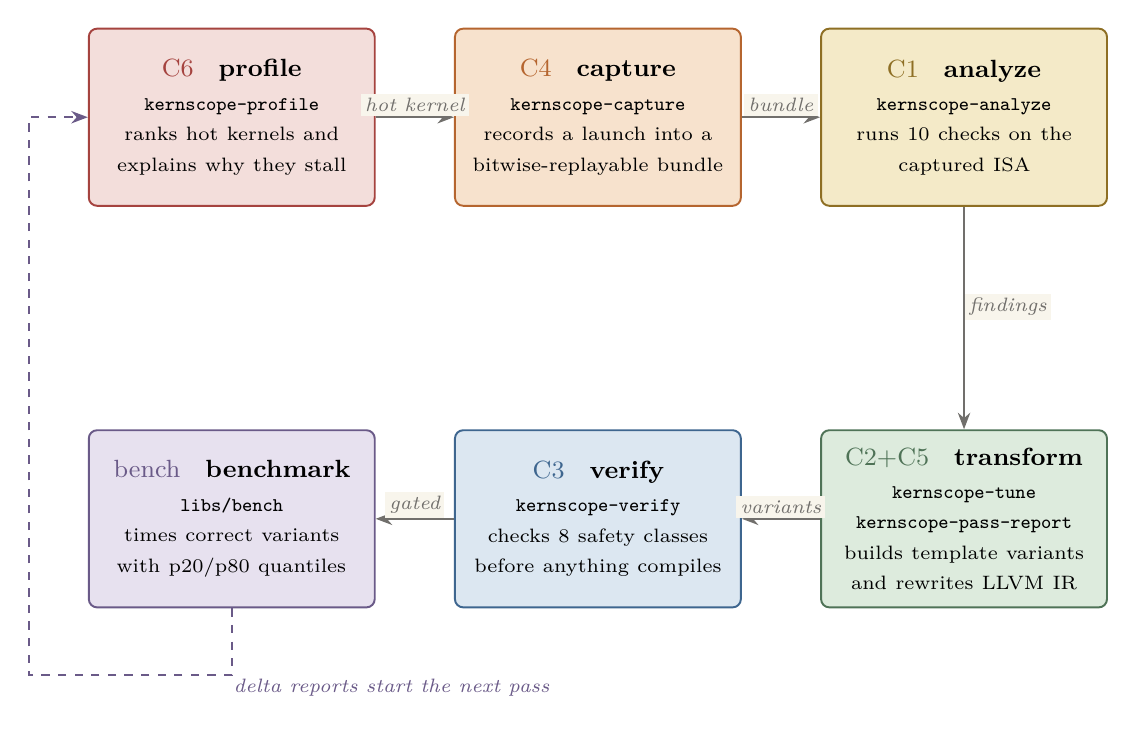
\begin{tikzpicture}[
    font=\small,
    card/.style={draw, rounded corners=3pt, align=center, text width=3.35cm,
                 minimum height=2.25cm, inner sep=4pt, line width=0.7pt},
    title/.style={font=\small\bfseries},
    cli/.style={font=\ttfamily\scriptsize},
    body/.style={font=\scriptsize, text=ink!80},
    flow/.style={-{Stealth[length=2.1mm]}, line width=0.8pt, draw=ink!65},
    feed/.style={-{Stealth[length=2.1mm]}, line width=0.8pt, dashed, draw=kviolet},
    lbl/.style={font=\scriptsize\itshape, text=ink!65, fill=paper, inner sep=1.5pt},
  ]

  % Top row: profile -> capture -> analyze.
  \node[card, fill=kredfill, draw=kred] (prof) at (0,0)
    {{\color{kred}C6}\quad\textbf{profile}\\[1pt]
     \texttt{\scriptsize kernscope-profile}\\[3pt]
     {\scriptsize ranks hot kernels and\\explains why they stall}};
  \node[card, fill=korangefill, draw=korange] (cap) at (4.65,0)
    {{\color{korange}C4}\quad\textbf{capture}\\[1pt]
     \texttt{\scriptsize kernscope-capture}\\[3pt]
     {\scriptsize records a launch into a\\bitwise-replayable bundle}};
  \node[card, fill=kgoldfill, draw=kgold] (ana) at (9.3,0)
    {{\color{kgold}C1}\quad\textbf{analyze}\\[1pt]
     \texttt{\scriptsize kernscope-analyze}\\[3pt]
     {\scriptsize runs 10 checks on the\\captured ISA}};

  % Bottom row, right to left: transform -> verify -> benchmark.
  \node[card, fill=kgreenfill, draw=kgreen] (trans) at (9.3,-5.1)
    {{\color{kgreen}C2+C5}\quad\textbf{transform}\\[1pt]
     \texttt{\scriptsize kernscope-tune}\\
     \texttt{\scriptsize kernscope-pass-report}\\[3pt]
     {\scriptsize builds template variants\\and rewrites LLVM IR}};
  \node[card, fill=kbluefill, draw=kblue] (ver) at (4.65,-5.1)
    {{\color{kblue}C3}\quad\textbf{verify}\\[1pt]
     \texttt{\scriptsize kernscope-verify}\\[3pt]
     {\scriptsize checks 8 safety classes\\before anything compiles}};
  \node[card, fill=kvioletfill, draw=kviolet] (bench) at (0,-5.1)
    {{\color{kviolet}bench}\quad\textbf{benchmark}\\[1pt]
     \texttt{\scriptsize libs/bench}\\[3pt]
     {\scriptsize times correct variants\\with p20/p80 quantiles}};

  % Forward path.
  \draw[flow] (prof.east) -- node[lbl, above] {hot kernel} (cap.west);
  \draw[flow] (cap.east) -- node[lbl, above] {bundle} (ana.west);
  \draw[flow] (ana.south) -- node[lbl, right, pos=0.45] {findings} (trans.north);
  \draw[flow] (trans.west) -- node[lbl, above] {variants} (ver.east);
  \draw[flow] (ver.west) -- node[lbl, above] {gated} (bench.east);

  % Delta feedback around the outside.
  \draw[feed] (bench.south) -- ++(0,-0.85) -| ($(prof.west)+(-0.75,0)$)
    -- (prof.west);
  \node[font=\scriptsize\itshape, text=kviolet, anchor=west] at (-0.1,-7.25)
    {delta reports start the next pass};

\end{tikzpicture}
}
\caption{The kernscope loop. The forward path is
profile $\rightarrow$ capture $\rightarrow$ analyze $\rightarrow$
transform/generate $\rightarrow$ verify $\rightarrow$ benchmark; the dashed
edge is the delta report that starts the next pass.}
\label{fig:loop}
\end{figure}

The loop is a convention over files and executables, not one monolithic
binary. \kst{scripts/demo.sh} runs five observable stages on the local
gfx1101: profile, capture, analyze, capture-tune, and verifier-gated tune plus
a pass delta. It writes \fpath{reports/demo/report.json} and a self-contained
HTML page, and it aborts early with a well-formed all-skipped report when
\fpath{/dev/kfd} is absent or \kst{KERNSCOPE_NO_GPU=1}. The committed run
completed in 153\,s against a 900\,s budget.

Six cross-tool edges make the loop more than a pipeline:
\begin{itemize}
  \item \textbf{profile $\rightarrow$ capture.} The profiler ranks hot kernels;
        capture records the hot one.
  \item \textbf{capture $\rightarrow$ analyze.} The analyzer runs on the
        captured kernel's disassembled ISA, not on a hand-picked example.
  \item \textbf{capture $\rightarrow$ tune.} \kst{kernscope-tune
        --from-capture} searches launch configurations over the bundle and
        validates each candidate bitwise.
  \item \textbf{tune $\rightarrow$ verify.} \kst{kernscope-tune --verify}
        gates variants before they are compiled.
  \item \textbf{pass $\rightarrow$ analyze.} \kst{kernscope-pass-report
        --report-pipeline} measures before/after deltas with the analyzer's
        own metrics.
  \item \textbf{profile $\leftrightarrow$ analyze.} The aggregated demo report
        links the profiler hint to the analyzer finding identifiers.
\end{itemize}

\subsection{The shared stack}
\label{sec:stack}

\begin{figure}[htbp]
\centering
\resizebox{\textwidth}{!}{% The shared stack: six tools, four library groups, and the external toolchain.
% The tools link only the groups they need; no tool links another tool.
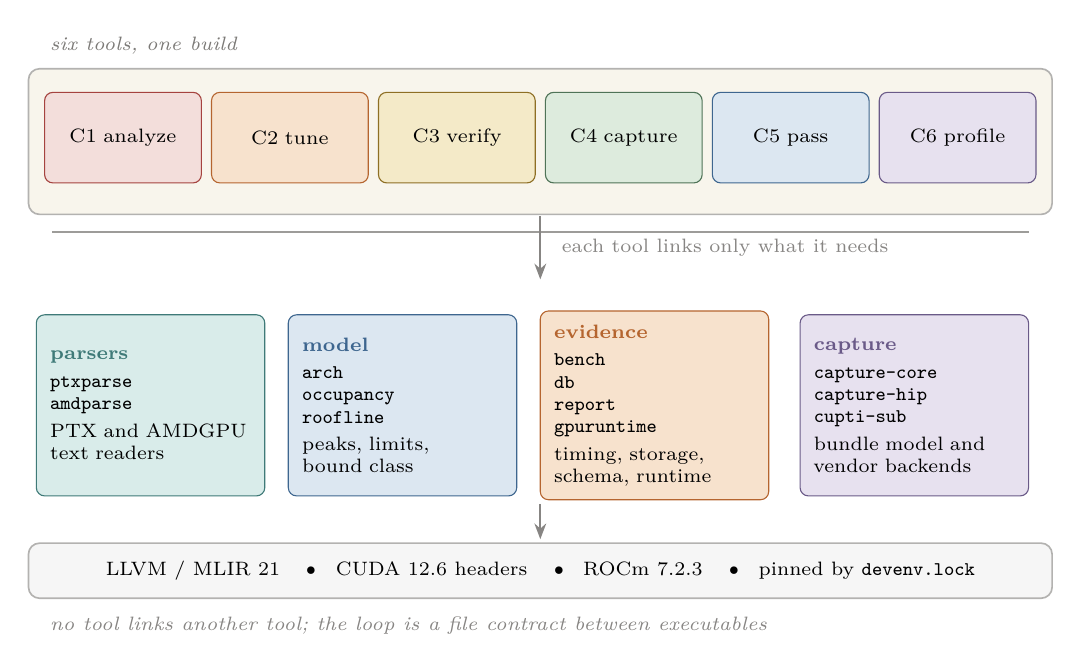
\begin{tikzpicture}[
    font=\small,
    band/.style={draw=ink!35, rounded corners=4pt, fill=paper, line width=0.6pt},
    tool/.style={draw, rounded corners=3pt, align=center, text width=1.85cm,
                 minimum height=1.15cm, inner sep=2pt, font=\scriptsize},
    group/.style={draw, rounded corners=3pt, align=left, text width=2.55cm,
                  minimum height=2.3cm, inner sep=5pt, font=\scriptsize},
    chip/.style={font=\ttfamily\scriptsize, text=ink!85},
    flow/.style={-{Stealth[length=2mm]}, line width=0.7pt, draw=ink!55},
  ]

  % Six tools in one band.
  \node[band, minimum width=13.0cm, minimum height=1.85cm] (tools) at (0,5.1) {};
  \node[font=\scriptsize\itshape, text=ink!60, anchor=west] at (-6.35,6.32)
    {six tools, one build};
  \foreach \x/\c/\f/\name in {
    -5.3/kred/kredfill/{C1 analyze},
    -3.18/korange/korangefill/{C2 tune},
    -1.06/kgold/kgoldfill/{C3 verify},
     1.06/kgreen/kgreenfill/{C4 capture},
     3.18/kblue/kbluefill/{C5 pass},
     5.3/kviolet/kvioletfill/{C6 profile}} {
    \node[tool, draw=\c, fill=\f] at (\x,5.15) {\name};
  }

  % Shared library groups.
  \node[group, draw=kteal, fill=ktealfill] (parsers) at (-4.95,1.75)
    {\textbf{\color{kteal}parsers}\\[2pt]
     \texttt{\scriptsize ptxparse}\\
     \texttt{\scriptsize amdparse}\\[2pt]
     {\scriptsize PTX and AMDGPU\\text readers}};
  \node[group, draw=kblue, fill=kbluefill] (model) at (-1.75,1.75)
    {\textbf{\color{kblue}model}\\[2pt]
     \texttt{\scriptsize arch}\\
     \texttt{\scriptsize occupancy}\\
     \texttt{\scriptsize roofline}\\[2pt]
     {\scriptsize peaks, limits,\\bound class}};
  \node[group, draw=korange, fill=korangefill] (evidence) at (1.45,1.75)
    {\textbf{\color{korange}evidence}\\[2pt]
     \texttt{\scriptsize bench}\\
     \texttt{\scriptsize db}\\
     \texttt{\scriptsize report}\\
     \texttt{\scriptsize gpuruntime}\\[2pt]
     {\scriptsize timing, storage,\\schema, runtime}};
  \node[group, draw=kviolet, fill=kvioletfill] (capture) at (4.75,1.75)
    {\textbf{\color{kviolet}capture}\\[2pt]
     \texttt{\scriptsize capture-core}\\
     \texttt{\scriptsize capture-hip}\\
     \texttt{\scriptsize cupti-sub}\\[2pt]
     {\scriptsize bundle model and\\vendor backends}};

  % One bracket carries the tools into the stack.
  \draw[ink!45, line width=0.6pt] (-6.2,3.95) -- (6.2,3.95);
  \draw[flow] (0,4.15) -- (0,3.35);
  \node[font=\scriptsize, text=ink!55, anchor=west] at (0.15,3.75)
    {each tool links only what it needs};

  % External toolchain.
  \node[band, minimum width=13.0cm, minimum height=0.7cm, fill=ink!4] (ext) at (0,-0.35)
    {\scriptsize LLVM / MLIR 21 \quad\(\bullet\)\quad CUDA 12.6 headers
     \quad\(\bullet\)\quad ROCm 7.2.3 \quad\(\bullet\)\quad pinned by \texttt{devenv.lock}};
  \draw[flow] (0,0.5) -- (0,0.05);

  % The rule that keeps the stack acyclic.
  \node[font=\scriptsize\itshape, text=ink!55, anchor=west] at (-6.35,-1.05)
    {no tool links another tool; the loop is a file contract between executables};
\end{tikzpicture}
}
\caption{The shared stack. Six tools sit over four library groups and the
LLVM/CUDA/ROCm toolchain. Each tool links only what it needs; no tool links
another tool.}
\label{fig:stack}
\end{figure}

The stack has twelve libraries in four functional groups. \term{Parsers}:
\kst{ptxparse}, \kst{amdparse}. \term{Model}: \kst{arch}, \kst{occupancy},
\kst{roofline}. \term{Evidence}: \kst{bench}, \kst{db}, \kst{report},
\kst{gpuruntime}. \term{Capture}: \kst{capture-core}, \kst{capture-hip},
\kst{cupti-sub}. The exact link graph, as built by CMake rather than as
sketched in the older notes, is in \Cref{tab:links}.

\begin{table}[htbp]
\centering
\small
\begin{tabularx}{\textwidth}{@{}l X@{}}
\toprule
Target & Direct dependencies \\
\midrule
\kst{kernscope-analyze} & \kst{kernscope::analyze}, \kst{kernscope::db}; the analyze library links \kst{ptxparse}, \kst{amdparse}, \kst{arch}, \kst{occupancy}, \kst{report}. \\
\kst{kernscope-tune} & \kst{tune_driver}, \kst{capture_tune}, \kst{report}; the driver links the three generators, \kst{arch}, \kst{occupancy}, \kst{roofline}, \kst{bench}, \kst{db}, \kst{gpuruntime}. \\
\kst{kernscope-verify} & LLVM only. \\
\kst{kernscope-capture} & \kst{capture_core}, \kst{db}, \kst{bench}, \kst{gpuruntime}, \kst{arch}; the HIP and CUPTI capture libraries are loaded as \kst{LD_PRELOAD} shared objects, not linked into the CLI. \\
\kst{kernscope-pass-report} & LLVM; the pass plugin is a separate \kst{MODULE}. \\
\kst{kernscope-profile} & \kst{profile_diag}, \kst{profile_enrich}, \kst{roofline}, \kst{report}, \kst{db}; \kst{profile_enrich} links \kst{occupancy}; the CUPTI and rocprofiler tracers are separate libraries. \\
\kst{kernscope-bench} & \kst{bench}, \kst{db}, \kst{gpuruntime}, \kst{arch}. \\
\bottomrule
\end{tabularx}
\caption{Direct CMake dependencies of the tool targets. ``LLVM only'' means the
tool does not link a \fpath{libs/} target.}
\label{tab:links}
\end{table}

\subsection{Evidence flow}
\label{sec:evidence-flow}

\begin{figure}[htbp]
\centering
\resizebox{\textwidth}{!}{% From tool output to the archival report: one schema, one provenance flag.
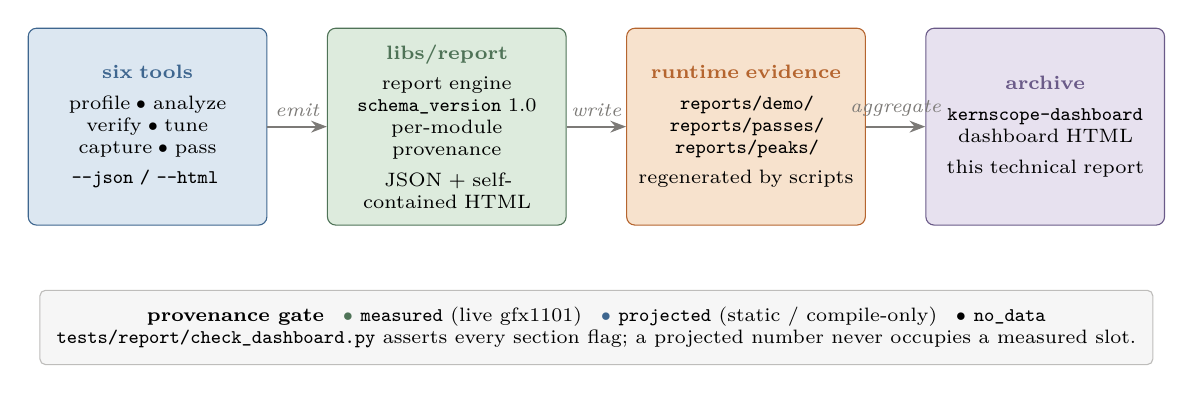
\begin{tikzpicture}[
    font=\small,
    box/.style={draw=ink!35, rounded corners=3pt, align=center, text width=2.75cm,
                minimum height=2.5cm, inner sep=4pt, font=\scriptsize, fill=paper},
    wide/.style={draw=ink!30, rounded corners=2pt, align=center, inner sep=6pt,
                 font=\scriptsize, fill=ink!4},
    flow/.style={-{Stealth[length=2mm]}, line width=0.8pt, draw=ink!60},
    lbl/.style={font=\scriptsize\itshape, text=ink!60},
  ]

  \node[box, fill=kbluefill, draw=kblue] (tools) at (0,0)
    {\textbf{\color{kblue}six tools}\\[3pt]
     profile \(\bullet\)\ analyze\\
     verify \(\bullet\)\ tune\\
     capture \(\bullet\)\ pass\\[3pt]
     {\scriptsize\ttfamily --json / --html}};
  \node[box, fill=kgreenfill, draw=kgreen] (engine) at (3.8,0)
    {\textbf{\color{kgreen}libs/report}\\[3pt]
     report engine\\
     \texttt{schema\_version} 1.0\\
     per-module\\provenance\\[3pt]
     JSON + self-contained HTML};
  \node[box, fill=korangefill, draw=korange] (runtime) at (7.6,0)
    {\textbf{\color{korange}runtime evidence}\\[3pt]
     \texttt{reports/demo/}\\
     \texttt{reports/passes/}\\
     \texttt{reports/peaks/}\\[3pt]
     regenerated by scripts};
  \node[box, fill=kvioletfill, draw=kviolet] (archive) at (11.4,0)
    {\textbf{\color{kviolet}archive}\\[3pt]
     \texttt{kernscope-dashboard}\\
     dashboard HTML\\[3pt]
     this technical report};

  \draw[flow] (tools) -- node[lbl, above] {emit} (engine);
  \draw[flow] (engine) -- node[lbl, above] {write} (runtime);
  \draw[flow] (runtime) -- node[lbl, above] {aggregate} (archive);

  \node[wide, minimum width=13.0cm] at (5.7,-2.55)
    {\textbf{provenance gate}\quad
     \textcolor{kgreen}{\(\bullet\)}~\texttt{measured} (live gfx1101)\quad
     \textcolor{kblue}{\(\bullet\)}~\texttt{projected} (static / compile-only)\quad
     \(\bullet\)~\texttt{no\_data}\\
     \texttt{tests/report/check\_dashboard.py} asserts every section flag;
     a projected number never occupies a measured slot.};
\end{tikzpicture}
}
\caption{Evidence flow. Tools emit report models through \fpath{libs/report};
the runtime artifacts are aggregated by the dashboard and frozen in this
report. The provenance gate is a convention plus a separate validator, not a
schema-enforced property.}
\label{fig:evidence}
\end{figure}

A tool report is a JSON document with a schema version and a provenance
object. The demo aggregator combines the five stages into one model and keeps
cross-tool links: the profiler hint carries the analyzer finding identifiers
and the stage-3 evidence path. The dashboard has six sections
(\kst{analyzer}, \kst{tune}, \kst{verify}, \kst{capture}, \kst{profile},
\kst{pass}), each with \kst{provenance.mode} and a \kst{measured} boolean.
\Cref{sec:provenance} states exactly what the schemas require and where the
provenance convention lives outside them.

\subsection{Build and repository shape}
\label{sec:build}

The project is a C++20 CMake superbuild. \fpath{CMakeLists.txt} requires
LLVM 21.1 and treats MLIR as optional; it applies \kst{-Wall -Wextra -Werror}
globally. \fpath{scripts/configure.sh} resolves \kst{LLVM_DIR} and
\kst{MLIR_DIR} from the nix store when the build is not already inside
\kst{devenv shell}. \fpath{devenv.nix} supplies LLVM/MLIR 21, the CUDA 12.6
redistributables, ROCm 7.2.3, gtest, lit, CMake, Ninja, and a Python with
NumPy and pytest. The build registers the libraries first, then the tools,
then the lit suite, so no tool can depend downward on another tool.

The repository keeps the source and the tests; the runtime evidence directory
is generated. This report is the committed archive of the evidence that was
present at consolidation time. Appendix~\ref{app:consolidation} records what
was folded here and what remains as a separate diagram asset.

% ===========================================================================
\section{Hardware and execution model}
\label{sec:hardware}

\subsection{The local live path}
\label{sec:local}

The development machine has one AMD Radeon RX 7800 XT (gfx1101, RDNA 3) and
no NVIDIA GPU. HIP code compiles with \kst{hipcc} and runs live; \fpath{/dev/kfd}
is the runtime gate. \kst{libs/arch} holds the measured machine peaks, the
per-architecture limits, and the occupancy constants. The peaks used by the
roofline engine are shown in \Cref{tab:peaks}; they were measured with
\kst{kernscope-bench} on 2026-08-14 with clocks recorded but not locked.

\begin{table}[htbp]
\centering
\small
\begin{tabular}{@{}llrr@{}}
\toprule
Family & Microbenchmark & Median & Derived peak \\
\midrule
\kst{peak_flops} & register-resident FFMA loop & 13.51\,ms & 16.32\,TFLOPS fp32 \\
\kst{peak_bw_read} & 512\,MiB DRAM read & 0.907\,ms & 591\,GB/s \\
\kst{peak_bw_d2d} & 1\,GiB device-to-device & 2.26--2.30\,ms & 467--475\,GB/s \\
\kst{peak_lds} & LDS read + write & 10.14--10.32\,ms & 9.7\,TB/s \\
\bottomrule
\end{tabular}
\caption{Measured gfx1101 peaks. All rows are \kst{provenance.mode=measured};
the ridge point used by the tuner and profiler is $16.32\times10^{12}/591\times10^{9}
= 27.61$ FLOP/byte.}
\label{tab:peaks}
\end{table}

\subsection{CUDA is compile-only here}
\label{sec:cuda-compile}

The CUDA path compiles kernels for sm\_80 and sm\_90 with \kst{nvcc} against
the CUDA 12.6 redistributables from the nix store. The resulting PTX and cubins
are analyzed and compiled, but no CUDA runtime executes on the machine.
\kst{libs/gpuruntime} provides a mock backend for the capture shim, and
\kst{libs/cupti-sub} compiles and unit-tests the CUPTI subscription against
synthetic activity records. The repository commits no NVIDIA headers: the nix
store resolves \kst{#include <cuda_occupancy.h>}-style names at build time,
and \kst{scripts/ci.sh} guards both filenames and content.

\begin{figure}[htbp]
\centering
\resizebox{\textwidth}{!}{% Three execution venues for one source tree.
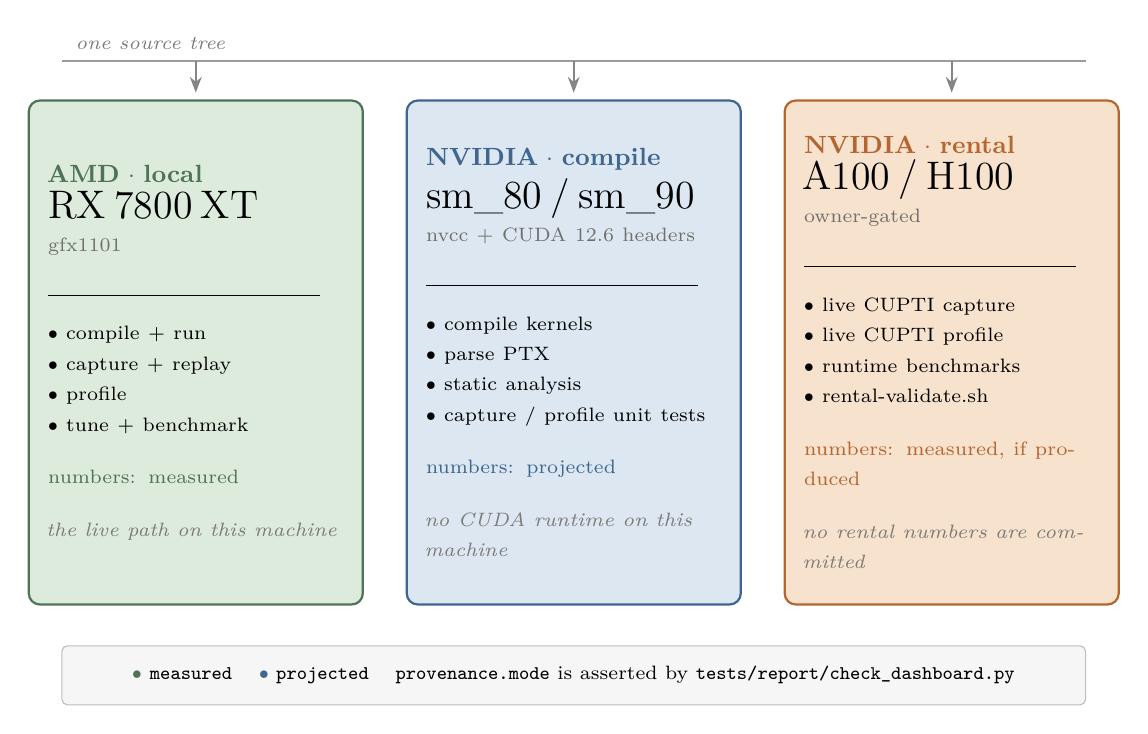
\begin{tikzpicture}[
    font=\small,
    venue/.style={draw, rounded corners=4pt, align=left, text width=3.75cm,
                  minimum height=6.4cm, inner sep=7pt, line width=0.8pt},
    flow/.style={-{Stealth[length=2mm]}, line width=0.7pt, draw=ink!55},
  ]

  % One source, three venues.
  \draw[ink!45, line width=0.6pt] (-6.5,4.45) -- (6.5,4.45);
  \node[font=\scriptsize\itshape, text=ink!60, anchor=west] at (-6.45,4.68)
    {one source tree};
  \foreach \x in {-4.8,0,4.8} {
    \draw[flow] (\x,4.45) -- (\x,4.05);
  }

  \node[venue, draw=kgreen, fill=kgreenfill] (amd) at (-4.8,0.75)
    {{\color{kgreen}\small\bfseries AMD \(\cdot\) local}\\[2pt]
     {\Large RX 7800 XT}\\[1pt]
     {\scriptsize\color{ink!65} gfx1101}\\[5pt]
     \rule{3.45cm}{0.3pt}\\[5pt]
     {\scriptsize\(\bullet\)~compile + run}\\
     {\scriptsize\(\bullet\)~capture + replay}\\
     {\scriptsize\(\bullet\)~profile}\\
     {\scriptsize\(\bullet\)~tune + benchmark}\\[8pt]
     {\color{kgreen}\scriptsize numbers: measured}\\[8pt]
     {\scriptsize\itshape\color{ink!60} the live path on this machine}};

  \node[venue, draw=kblue, fill=kbluefill] (cuda) at (0,0.75)
    {{\color{kblue}\small\bfseries NVIDIA \(\cdot\) compile}\\[2pt]
     {\Large sm\_80 / sm\_90}\\[1pt]
     {\scriptsize\color{ink!65} nvcc + CUDA 12.6 headers}\\[5pt]
     \rule{3.45cm}{0.3pt}\\[5pt]
     {\scriptsize\(\bullet\)~compile kernels}\\
     {\scriptsize\(\bullet\)~parse PTX}\\
     {\scriptsize\(\bullet\)~static analysis}\\
     {\scriptsize\(\bullet\)~capture / profile unit tests}\\[8pt]
     {\color{kblue}\scriptsize numbers: projected}\\[8pt]
     {\scriptsize\itshape\color{ink!60} no CUDA runtime on this machine}};

  \node[venue, draw=korange, fill=korangefill] (rental) at (4.8,0.75)
    {{\color{korange}\small\bfseries NVIDIA \(\cdot\) rental}\\[2pt]
     {\Large A100 / H100}\\[1pt]
     {\scriptsize\color{ink!65} owner-gated}\\[5pt]
     \rule{3.45cm}{0.3pt}\\[5pt]
     {\scriptsize\(\bullet\)~live CUPTI capture}\\
     {\scriptsize\(\bullet\)~live CUPTI profile}\\
     {\scriptsize\(\bullet\)~runtime benchmarks}\\
     {\scriptsize\(\bullet\)~rental-validate.sh}\\[8pt]
     {\color{korange}\scriptsize numbers: measured, if produced}\\[8pt]
     {\scriptsize\itshape\color{ink!60} no rental numbers are committed}};

  % Provenance banner.
  \node[draw=ink!30, rounded corners=2pt, fill=ink!4, minimum width=13.0cm,
        minimum height=0.75cm, align=center, font=\scriptsize] at (0,-3.35)
    {\textcolor{kgreen}{\(\bullet\)}~\texttt{measured} \quad
     \textcolor{kblue}{\(\bullet\)}~\texttt{projected} \quad
     \texttt{provenance.mode} is asserted by
     \texttt{tests/report/check\_dashboard.py}};
\end{tikzpicture}
}
\caption{Three execution venues. The AMD column is live and measured, the
NVIDIA compile column is projected, and the rental column is owner-gated and
currently has no committed numbers.}
\label{fig:venues}
\end{figure}

\subsection{The rental gate}
\label{sec:rental}

Live NVIDIA capture and profiling run only on a rented A100/H100-class host
through \fpath{scripts/rental-validate.sh}. The script is never called by
\kst{ci.sh} and refuses to run when \kst{CI=true}. It prints the command
sequence in \kst{--dry-run} mode, then, in exec mode, checks the build tree,
probes CUDA and CUPTI, runs the \kst{gpu-nvidia-rental} tests, and writes a
timestamped summary under \fpath{reports/rentals/}. Gating is procedural, not
authenticated: the script checks the environment, not the identity of the
operator. The repository held no rental numbers at consolidation time.

\subsection{Capture mechanisms}
\label{sec:capture-mechanisms}

The three capture mechanisms share the \fpath{libs/capture-core} session
model and \kst{BundleWriter}. This is what makes a bundle written by any
mechanism parse identically.

\begin{table}[htbp]
\centering
\small
\begin{tabularx}{\textwidth}{@{}l l l X@{}}
\toprule
Mechanism & Vendor & Local status & Transport and scope \\
\midrule
CUPTI callback/injection & NVIDIA & compile + unit only; rental-gated live & \kst{CUDA_INJECTION64_PATH} or direct \kst{libcupti.so}; Memory4 allocation records; \kst{cuFuncGetParamInfo}; module-load callback. \\
LD\_PRELOAD shim & NVIDIA & compile + unit; mock runtime locally & PLT interposition of \kst{cuda*}/\kst{cu*}; \kst{cudaMalloc}/\kst{cudaFree}; fatbin/\kst{cuModuleLoadData}. \\
rocprofiler-sdk intercept & AMD & live on gfx1101 & \kst{LD_PRELOAD} plus intercept tables; HIP allocations; AMDGPU metadata; hsaco code objects; bitwise replay validated. \\
\bottomrule
\end{tabularx}
\caption{Capture mechanisms and their local status. The NVIDIA paths never run
live on this machine.}
\label{tab:capture-mechanisms}
\end{table}

\subsection{The CUDA 13 migration surface}
\label{sec:cuda13}

The suite pins CUDA 12.6 and \kst{CUPTI_API_VERSION} 24. The CUDA 13 surface
is documented so that a header bump is a compile error at one place, not a
silent parse shift. The single place that reads raw CUPTI activity records is
\fpath{tools/profile/include/kernscope/profile/record_adapter.h}.

\begin{itemize}
  \item \textbf{Kernel records.} CUDA 12.x delivers
        \kst{CUpti_ActivityKernel9}; 13.x delivers \kst{CUpti_ActivityKernel10}.
        The 12.x struct moves to \kst{cupti_activity_deprecated.h}. Kernel10 is
        Kernel9 plus a tail \kst{uint8_t isDeviceLaunched} (and three padding
        bytes). The parser is a template over the delivered struct, selected by
        \kst{CUPTI_API_VERSION}; offsets are pinned by \kst{static_assert}s and
        \kst{isDeviceLaunched} is read by SFINAE, so a 12.x build compiles
        against Kernel9 and treats the absent field as zero.
  \item \textbf{Removed APIs.} The CUPTI Event API and Metric API are removed
        in CUDA 13 and return
        \kst{CUPTI_ERROR_LEGACY_PROFILER_NOT_SUPPORTED} (38). The PC-sampling
        ACTIVITY kind is replaced by \kst{cupti_pcsampling.h}. nvprof and the
        NVIDIA Visual Profiler are gone. The build forbids the Event and Metric
        APIs; all profiling data comes from the Activity API.
  \item \textbf{Replacements.} The Profiling API and PerfWorks Metric API are
        replaced by the CUPTI Range Profiling API and the Profiler Host API.
        Multi-subscriber V2 APIs arrive in CUDA 13.3+; the 12.x
        single-subscriber path in \kst{libs/cupti-sub} degrades to the fallback
        when a second subscriber is active.
  \item \textbf{Record-kind discipline.} Only
        \kst{CUPTI_ACTIVITY_KIND_CONCURRENT_KERNEL} (10) is enabled. The
        serializing \kst{KERNEL} kind (3) changes collection behavior and is
        never used.
  \item \textbf{Version codes.} \kst{CUPTI_API_VERSION} 24 corresponds to CUDA
        12.6; CUDA 13.0 reports 130001.
\end{itemize}

\subsection{What the hardware split implies}
\label{sec:hardware-implies}

The local machine can measure HIP behavior, PTX text analysis, static IR
verification, and compile-only CUDA artifacts. It cannot measure NVIDIA
runtime behavior. Every performance number in this report is therefore one of:
a live gfx1101 measurement, a static projection from IR or PTX, or a
correctness result from a compile gate. \Cref{sec:eval} keeps those categories
separate.

% ===========================================================================
\section{The shared libraries}
\label{sec:libs}

\subsection{Architecture database and record store}
\label{sec:arch-lib}

\kst{libs/arch} is an interface library of per-architecture constants: SM
counts, register file sizes, shared-memory budgets, warp widths, and the
measured gfx1101 peaks. It is the only place that answers ``how big is the
register file on this part.'' \kst{libs/db} is the JSONL record store. Records
are keyed by \kst{gpu_arch}, \kst{kernel_family}, and a shape hash, and the
store supports \kst{query_best} over the recorded timings. The tune cache and
the benchmark/replay records both use it.

\subsection{PTX and AMDGPU parsers}
\label{sec:parsers}

\kst{libs/ptxparse} is a hand-written PTX lexer and parser: modules, entry
functions, register declarations, instructions, and operand forms. It is used
by the analyzer, the pass delta, and the auxiliary PTX dump source.
\kst{libs/amdparse} uses LLVM 21's MC layer to parse AMDGPU assembly and
recover instruction, register, and operand facts. Both parsers preserve enough
source text for the analyzer to emit evidence paths and finding identifiers.

\subsection{Occupancy and roofline}
\label{sec:occ-roof}

\kst{libs/occupancy} implements the min-wins occupancy model. For a block size
and a kernel's register and shared-memory demand it computes resident blocks
per SM from the thread, warp, shared-memory, register, and hard block limits,
then reports the binding limiter. The NVIDIA register limit uses the
architecture's allocation granularity:
\[
  \text{blocks}_{\text{regs}} =
  \left\lfloor \frac{65536}{\text{granule}(\text{regs per thread}) \times
  \text{threads per block}} \right\rfloor .
\]
The AMD path models waves per SIMD and SIMD count, with the RDNA 3 VGPR file
resolution described in the project notes. Occupancy is explicitly theoretical:
it does not predict achieved occupancy under memory stalls.

\kst{libs/roofline} computes arithmetic intensity, the ridge point, the
compute and memory ceilings, the bound class, and a position in $(0,1]$:
\[
  \text{position} = \min\!\left(1, \frac{\text{AI}}{\text{ridge}}\right),
  \qquad
  \text{ridge} = \frac{\text{peak FLOP/s}}{\text{peak bytes/s}} .
\]
The engine refuses to produce a position when the architecture has no measured
peaks; \kst{roofline.ok} is false rather than a datasheet guess.

\subsection{Benchmark harness and runtime shim}
\label{sec:bench-lib}

\kst{libs/bench} implements time-based warmup and repetition budgets, an L2
flush between trials, adaptive trial counts, and median plus p20/p80
quantiles. It is the timing method for the tuner, capture replay benchmark,
and peak microbenchmarks. \kst{libs/gpuruntime} is a thin CUDA/HIP runtime
wrapper. It exposes the allocation, copy, launch, and synchronization surface
the capture and replay code needs, with compile-only CUDA and mock backends so
the shim can be exercised without an NVIDIA device.

\subsection{Report engine and provenance}
\label{sec:report-lib}

\kst{libs/report} writes the self-contained JSON and HTML report form used by
the tools. It sets \kst{schema_version} to \kst{"1.0"} and provides the
per-module provenance object with a \kst{mode} and a \kst{measured} boolean.
The report is self-contained: inline CSS and JavaScript, no external assets,
and an embedded JSON payload under a stable script identifier, so a checker can
extract and validate it without network access.

\subsection{Capture backends}
\label{sec:capture-libs}

\kst{libs/capture-core} owns the session model, the event log, the bundle
writer and reader, the VA-faithful snapshot policy, and the patch table. It
also builds the NVIDIA LD\_PRELOAD shim and a mock CUDA runtime used by the
unit tests. \kst{libs/capture-hip} is the AMD shared object: it registers
rocprofiler-sdk intercept tables, records dispatches and code objects, and
writes the same bundle model. \kst{libs/cupti-sub} is the shared CUPTI
subscription layer used by the NVIDIA capture path and the profiler; it
enforces a single-tool scope contract because the 12.x CUPTI subscription is
single-subscriber.

\subsection{Dependency rules}
\label{sec:deps}

Nothing in \fpath{libs/} depends on a tool. The tools link libraries, not each
other. The only cross-tool relationships are runtime file contracts: a bundle
written by capture, a report written by a tool, a JSONL record written by the
tuner. This is why the loop can be exercised by separate executables and why a
tool can be replaced without rebuilding the stack.

% ===========================================================================

% ===========================================================================
\clearpage
\floraon
\florathispage{layout=surround, seed=37, density=0.32, visitors=0.08}
\part{The tools}
\thispagestyle{empty}
\clearpage
\floraoff
% ===========================================================================

\section{C1: static analyzer}
\label{sec:c1}

\kst{kernscope-analyze} consumes PTX or AMDGPU assembly text and emits one
kernel report plus a suggestion list. It is a static tool: it estimates
occupancy and memory behavior from the instruction stream and the architecture
database, and it labels every estimate as a metric rather than a measurement.

\subsection{Inputs, CLI, and precedence}
\label{sec:c1-cli}

\begin{lstlisting}
kernscope-analyze <file.ptx|file.s|file.isa> [options]
  --arch <sm_XX|gfxXXXX>   required for AMDGPU; PTX defaults to .target
  --block <N>              launch block size for occupancy
  --json | --text | --html output format (default --text)
  --source <file.cu|file.hip>  source stem for the kernel label
  --version | --help
\end{lstlisting}

The analyzer recognizes \kst{sm_75}, \kst{sm_80}, \kst{sm_86}, \kst{sm_89},
\kst{sm_90}, \kst{sm_100}, \kst{sm_120}, \kst{gfx90a}, \kst{gfx942}, and
\kst{gfx1101}. A \kst{.ptx} file goes through the PTX parser; \kst{.s} and
\kst{.isa} files go through the AMDGPU parser; other extensions are
content-sniffed. A directory input may carry \kst{manifest.json} with
\kst{arch}, \kst{block_size}, and a \kst{ptxas_v_report}; command-line flags
override the manifest. Without \kst{--block}, occupancy emits the
\kst{block_size_unknown} diagnostic rather than guessing.

Register pressure prefers \kst{ptxas -v} when a report is supplied. Otherwise
the analyzer uses the declared \kst{.reg} counts plus the \kst{.local} frame,
an upper bound: ptxas can reuse registers, so the proxy can overestimate.
The AMDGPU path uses \kst{scratch_load} and \kst{scratch_store} for spills and
does not have a \kst{next_free_vgpr} value in plain assembly, so it does not
invent one.

\subsection{The ten analyses}
\label{sec:c1-checks}

\begin{table}[htbp]
\centering
\small
\begin{tabularx}{\textwidth}{@{}l X l@{}}
\toprule
Analysis & What it computes & Finding \\
\midrule
Register pressure & Per-thread registers, warp allocation, local frame. & \kst{spill}, \kst{cannot_estimate_registers} \\
Occupancy + limiter & Blocks per SM from thread, warp, smem, register, and hard limits. & \kst{occupancy}, \kst{limiter} \\
Global coalescing & 128\,B sectors, used versus transferred bytes per warp. & \kst{coalescing}, \kst{coalescing_unknown} \\
Shared banks & Bank index, distinct banks, conflict way. & \kst{bank_conflict}, \kst{bank_conflict_unknown} \\
Warp divergence & Branch target and post-dominator analysis over thread-dependent predicates. & \kst{possibly_divergent_branch}, \kst{divergent_inner_loop} \\
Barriers & \kst{bar.sync}, \kst{bar.warp}, cluster barriers, density per loop, reachability under divergence. & \kst{divergent_barrier} \\
Instruction mix & FP32/FP16/INT/LSU/SMEM/tensor/control histogram. & \kst{mix_count_*}, \kst{mix_pct_*} \\
Tensor cores & PTX \kst{mma}/\kst{wmma}/\kst{wgmma}/\kst{tcgen05}; AMD \kst{v_mfma_*}/\kst{v_wmma_*}. & \kst{no_tensor_core_usage}, \kst{tensor_ops} \\
Spills & \kst{ld.local}/\kst{st.local}, local frame bytes, AMD scratch ops. & \kst{spill}, \kst{spill_bytes} \\
Latency & Static critical-path estimate from microbenchmark-derived op latencies. & \kst{latency_bottleneck}, \kst{latency_unknown_arch} \\
\bottomrule
\end{tabularx}
\caption{The analyzer's ten analyses. The occupancy model is the min-wins
formula from the occupancy library; the latency estimate is explicitly
approximate.}
\label{tab:c1checks}
\end{table}

The occupancy estimate is:
\[
  \text{blocks} = \min\left(
  \left\lfloor \frac{\text{threads}_{\max}}{\text{threads per block}}\right\rfloor,
  \left\lfloor \frac{\text{warps}_{\max}}{\text{warps per block}}\right\rfloor,
  \left\lfloor \frac{\text{smem}_{\max}}{\text{smem per block}}\right\rfloor,
  \text{blocks}_{\text{regs}},
  \text{blocks}_{\text{hard}}
  \right),
\]
and the binding term is reported as the limiter. The bank-conflict metric
uses $32$ banks of $4$ bytes: the bank index is
$(\text{word} \div 4) \bmod 32$, and the conflict way is lanes divided by
distinct banks. Coalescing uses the 128-byte-sector model and reports a
byte-efficiency ratio; it does not claim a hardware counter.

\subsection{Suggestion rules}
\label{sec:c1-suggest}

The suggestion engine owns \kst{report.suggestions}. It clears the list and
emits at most one suggestion per triggering finding, in a fixed priority
order, with an evidence text and a \kst{triggered_by} link.

\begin{table}[htbp]
\centering
\small
\begin{tabularx}{\textwidth}{@{}l X l@{}}
\toprule
Rule & Trigger and recommendation & Evidence \\
\midrule
\kst{tile_k_32} & Bank conflict of way $\ge 2$; set the shared tile to 32 words. & Current stride, banks, shared bytes \\
\kst{split_accumulator} & Register limiter and at least 16 FP32 FMAs; split the accumulator. & Registers, FMA count, fragment size \\
\kst{hoist_predicate} & Divergent branch inside an inner loop; hoist the predicate. & Branch site, predicate dependence \\
\kst{vectorize_coalescing} & Coalescing efficiency below 1.0 and no bank conflict; target 128\,B per warp. & Efficiency, sectors, vector width \\
\bottomrule
\end{tabularx}
\caption{Suggestion rules. The priority order is the table order. The engine
drops instruction-mix informational findings so a suggestion is tied to an
actionable warning.}
\label{tab:c1suggest}
\end{table}

\subsection{Report and golden result}
\label{sec:c1-evidence}

The report is a JSON object with \kst{kernel}, \kst{metrics}, \kst{limiter},
\kst{warnings}, and \kst{suggestions}; the schema is summarized in
Appendix~\ref{app:report-schema}. The committed golden fixture is a
fused-attention-style CUDA kernel whose PTX targets sm\_86:
occupancy $9 \text{ blocks} \times 2 \text{ warps} / 48 = 0.375$, limiter
\kst{registers}, 102 registers per thread, coalescing efficiency $0.5$,
a $68$-word shared stride that maps to banks $\{0,4,\dots,28\}$ with way $4$,
two \kst{bar.sync} instructions, 1024 FP32 FMAs, zero spills, and three
warnings plus three suggestions. The sm\_86 fixture is a parser corpus
artifact; it is independent of the local \kst{nvcc} capability pin.

% ===========================================================================
\section{C2: correctness-gated autotuner}
\label{sec:c2}

\kst{kernscope-tune} searches a kernel family's configuration grid for the
fastest variant that passes a bf16 golden gate. It reports the winner with
roofline and occupancy evidence, the full variant list, and a reproducibility
bundle. It is not a blind search: infeasible configurations are rejected
before compilation, and wrong kernels are never benchmarked.

\subsection{Families and search spaces}
\label{sec:c2-space}

\begin{table}[htbp]
\centering
\small
\begin{tabularx}{\textwidth}{@{}l X@{}}
\toprule
Family & Auto grid \\
\midrule
\kst{matmul} & $(BM,BN) \in \{(64,64),(128,128)\} \times BK \in \{16,32\} \times
warps \in \{1,2,4\} \times stages \in \{1,2\}$: 24 configs. The full grid
expands to 4608 combinations over $BK$ 8--64, stages 1--4, vector width 1--4,
XOR swizzle, and unroll 1--4. \\
\kst{bias_gelu}, \kst{softmax}, \kst{layernorm}, \kst{reduction} &
block $\in \{128,256,512,1024\}$ $\times$ vector width $\in \{1,2,4,8\}$;
softmax and layernorm add a one-pass/two-pass mode, reduction adds
strided/tree. \\
\kst{flash_attention} & $Br \times Bc \in \{32,64\}^2$ $\times$ stages
$\{1,2\}$ $\times$ vector width $\{1,2,4\}$ $\times$ shared-memory layout
(padding/XOR) $\times$ causal on/off. \\
\bottomrule
\end{tabularx}
\caption{Tuner families and their search spaces.}
\label{tab:c2space}
\end{table}

Each family owns a template generator that validates membership in the search
space and checks the \fpath{libs/arch} budgets (registers, shared memory,
warp/block divisibility, vector tiling) before compilation. A rejection is a
reason string, not a compiler error.

\subsection{The pipeline}
\label{sec:c2-pipeline}

\begin{figure}[htbp]
\centering
\resizebox{\textwidth}{!}{% Tuner pipeline: template path and capture path.
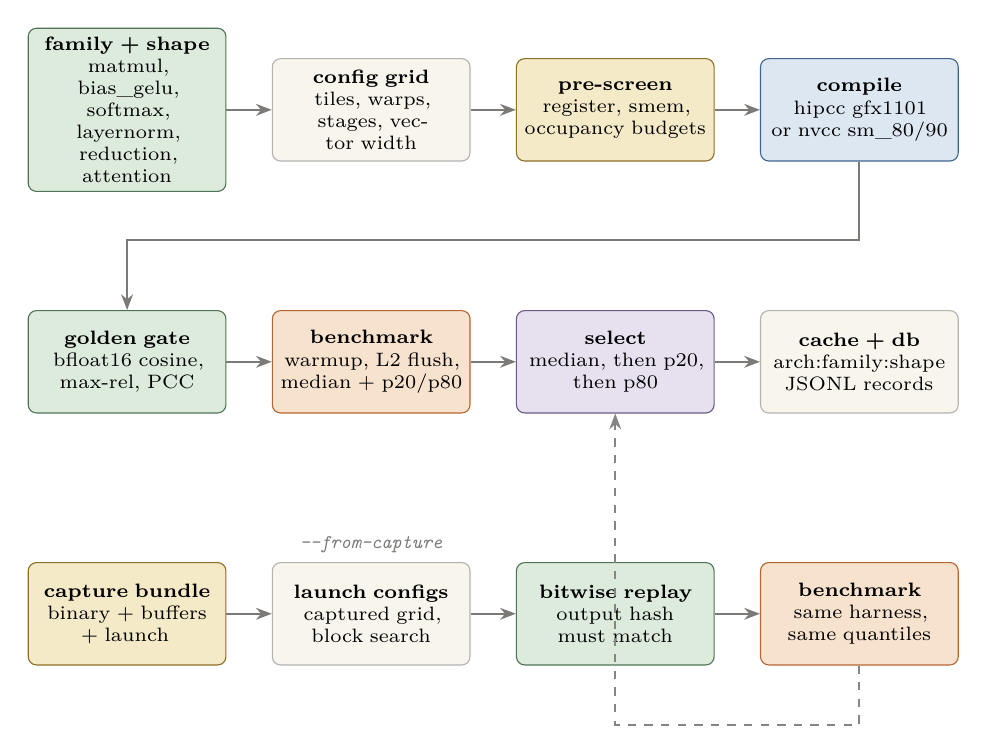
\begin{tikzpicture}[
    font=\small,
    box/.style={draw=ink!35, rounded corners=3pt, align=center, text width=2.3cm,
                minimum height=1.3cm, inner sep=3pt, font=\scriptsize, fill=paper},
    flow/.style={-{Stealth[length=2mm]}, line width=0.8pt, draw=ink!60},
    dflow/.style={-{Stealth[length=2mm]}, line width=0.7pt, dashed, draw=ink!55},
    lbl/.style={font=\scriptsize\itshape, text=ink!60},
  ]

  % Template path.
  \node[box, fill=kgreenfill, draw=kgreen] (family) at (0,2.1)
    {\textbf{family + shape}\\matmul, bias\_gelu,\\softmax, layernorm,\\reduction, attention};
  \node[box, fill=paper] (grid) at (3.1,2.1)
    {\textbf{config grid}\\tiles, warps,\\stages, vector width};
  \node[box, fill=kgoldfill, draw=kgold] (screen) at (6.2,2.1)
    {\textbf{pre-screen}\\register, smem,\\occupancy budgets};
  \node[box, fill=kbluefill, draw=kblue] (compile) at (9.3,2.1)
    {\textbf{compile}\\hipcc gfx1101\\or nvcc sm\_80/90};

  \draw[flow] (family) -- (grid);
  \draw[flow] (grid) -- (screen);
  \draw[flow] (screen) -- (compile);

  % The rest wraps to a second row.
  \node[box, fill=kgreenfill, draw=kgreen] (golden) at (0,-1.1)
    {\textbf{golden gate}\\bfloat16 cosine,\\max-rel, PCC};
  \node[box, fill=korangefill, draw=korange] (bench) at (3.1,-1.1)
    {\textbf{benchmark}\\warmup, L2 flush,\\median + p20/p80};
  \node[box, fill=kvioletfill, draw=kviolet] (select) at (6.2,-1.1)
    {\textbf{select}\\median, then p20,\\then p80};
  \node[box, fill=paper] (cache) at (9.3,-1.1)
    {\textbf{cache + db}\\arch:family:shape\\JSONL records};

  \draw[flow] (compile.south) -- ++(0,-1.0) -| (golden.north);
  \draw[flow] (golden) -- (bench);
  \draw[flow] (bench) -- (select);
  \draw[flow] (select) -- (cache);

  % Capture path.
  \node[box, fill=kgoldfill, draw=kgold] (bundle) at (0,-4.3)
    {\textbf{capture bundle}\\binary + buffers\\+ launch};
  \node[box, fill=paper] (launch) at (3.1,-4.3)
    {\textbf{launch configs}\\captured grid,\\block search};
  \node[box, fill=kgreenfill, draw=kgreen] (replay) at (6.2,-4.3)
    {\textbf{bitwise replay}\\output hash\\must match};
  \node[box, fill=korangefill, draw=korange] (cbench) at (9.3,-4.3)
    {\textbf{benchmark}\\same harness,\\same quantiles};

  \draw[flow] (bundle) -- (launch);
  \draw[flow] (launch) -- (replay);
  \draw[flow] (replay) -- (cbench);
  \node[lbl, above] at (3.1,-3.65) {\texttt{--from-capture}};

  % Shared selection.
  \draw[dflow] (cbench.south) -- ++(0,-0.75) -| (select.south);

\end{tikzpicture}
}
\caption{The tuner pipeline. The template path searches source variants;
the capture path searches launch configurations over a captured binary. Both
use the same benchmark and selection rules.}
\label{fig:tuner}
\end{figure}

A candidate moves through five stages:
\begin{enumerate}
  \item \textbf{Cache hit.} A config already in the tunecache is replayed
        without compiling.
  \item \textbf{GPU-free pre-screen.} The generator validates the config, then
        \kst{libs/occupancy} rejects zero-resident-block configs and configs
        below \kst{--min-occupancy}.
  \item \textbf{Compile.} The family generator emits a single-source
        \kst{.hip} file; \kst{hipcc --genco} compiles it for gfxXXXX, or
        \kst{nvcc -c} for sm\_XX.
  \item \textbf{Golden gate.} The kernel runs on the live HIP device through
        the template runner and the bf16 reference. The gate passes only when
        cosine $\ge 0.999$, maximum relative error $\le 10^{-2}$, and PCC
        $\ge 0.99$. A failure discards the variant; it is never timed.
  \item \textbf{Benchmark and select.} \fpath{libs/bench} warms up, flushes
        L2, adapts the trial count, and reports median and p20/p80. The best
        config wins by median, with p20, p80, and enumeration order as
        tie-breakers.
\end{enumerate}

The gate shape is the family's golden shape (64$^3$ for matmul), deliberately
decoupled from the benchmark shape. The cache is keyed
\kst{gpu_arch:family:shape_hash} and stamped with the minimum-occupancy floor
that produced it, so a floor-1.0 entry never replays for a floor-0.0 run.
\kst{--no-cache} skips the read but still writes the new entries.

\subsection{Outputs and reproducibility}
\label{sec:c2-output}

\kst{--json} emits the best config and timings, the baseline (the first
enumerated measured config), the speedup over that baseline, every measured
variant sorted by median, the pipeline counts, the roofline position and bound,
and the winning occupancy and limiter. \kst{--text} is the owner-facing
one-screen form. \kst{--html} is a self-contained variant comparison with the
model embedded under \kst{report-data} and the evidence under
\kst{tune-evidence}.

\kst{--emit-repro} writes a standalone directory with \kst{run.sh},
\kst{README.md}, and the winning config. The script regenerates the source,
repeats the exact compile command, and re-runs the golden gate at the winning
geometry. The nixpkgs revision from \kst{devenv.lock} is embedded and checked
against \kst{KERNSCOPE_EXPECT_NIXPKGS_REV} as a warning. The repro path needs
a live HIP device and exists for matmul plus the four elementwise families;
\kst{flash_attention} has no generator CLI and is rejected with a clear
message.

\subsection{Capture-tune mode}
\label{sec:c2-capture}

A capture bundle contains a binary, arguments, and buffers, but no source.
Template tuning cannot consume it; the launch configuration is the only
searchable degree of freedom. \kst{kernscope-tune --from-capture} restores the
captured launch, enumerates block sizes at the captured grid, pre-screens the
limits (threads per block $\le 1024$, grid x $\le 2^{31}-1$, grid y/z
$\le 65535$, shared memory within the architecture budget), replays each
survivor bitwise, and times only the survivors. The captured baseline is
candidate 1, so \kst{best.speedup} is always at least 1.0. The record key is
\kst{(arch, sha256(kernel name), sha256(bundle identity))}; the binary and
buffers stay byte-identical to the capture.

\subsection{Measured evidence}
\label{sec:c2-evidence}

In the demo, capture-tune explored four candidates over the captured
layernorm bundle. All four validated bitwise; the best block was 256 with a
median of $0.01206$\,ms against a $0.01208$\,ms baseline, a speedup of
$1.0017\times$. The verifier-gated template run on bias\_gelu at
$4096 \times 4096$ enumerated 13 variants, compiled 12, and gated one before
compilation. The best config (block 256, vector width 4) ran at
$0.17184$\,ms against a $0.20332$\,ms baseline, a $1.1832\times$ speedup,
occupancy 1 (limiter registers), arithmetic intensity 2.333, and roofline
position 0.0845 in the memory-bound class.

The dashboard records a separate measured matmul search with 15 variants, a
best median of $415.324\,\mu$s, and a worst median of $3.106$\,ms. The
per-run JSONL for that search is not committed, so the report quotes the
dashboard value and labels it as such rather than reconstructing a raw record.

% ===========================================================================
\section{C3: static verifier}
\label{sec:c3}

\kst{kernscope-verify} compiles CUDA or HIP source to LLVM IR at \kst{-O1}
and applies eight may-analyses. It does not prove a kernel correct; it proves
specific bounds and ordering facts when it can, and it refuses approval when
it cannot.

\subsection{Ingestion and launch tiers}
\label{sec:c3-ingest}

By default the host and device halves are compiled separately and linked into
one module, so the launch site is visible. The host pass supplies the launch
configuration through the \kst{__cudaPushCallConfiguration} or
\kst{cudaLaunchKernel} call. HIP uses clang 21 with \kst{--hip-path}.
\kst{--device-only} is a degraded mode: launch dimensions are lost unless the
kernel carries \kst{__launch_bounds__}.

Launch dimensions resolve into three tiers:
\begin{enumerate}
  \item \textbf{Exact}: constant dimensions at the launch site, giving exact
        ranges for \kst{threadIdx} and \kst{blockIdx}.
  \item \textbf{UpperBound}: \kst{__launch_bounds__} or \kst{nvvm.maxntid}
        provides a sound upper bound on \kst{blockDim}.
  \item \textbf{Symbolic}: runtime dimensions produce a \kst{SYMBOLIC_DIMS}
        verdict and a runtime-check suggestion, never a claim of safety.
\end{enumerate}

\begin{figure}[htbp]
\centering
\resizebox{\textwidth}{!}{% Verifier pipeline: source to verdicts to approved IR.
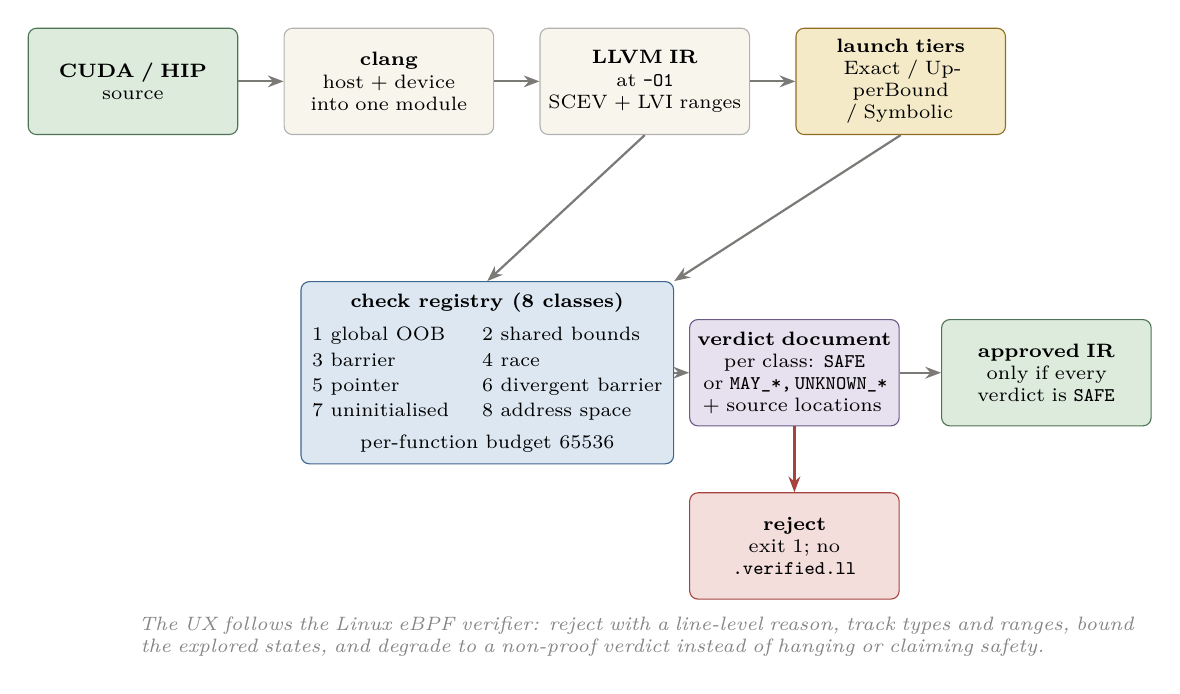
\begin{tikzpicture}[
    font=\small,
    box/.style={draw=ink!35, rounded corners=3pt, align=center, text width=2.45cm,
                minimum height=1.35cm, inner sep=3pt, font=\scriptsize, fill=paper},
    checks/.style={draw=kblue, rounded corners=3pt, align=center, inner sep=4pt,
                   font=\scriptsize, fill=kbluefill},
    flow/.style={-{Stealth[length=2mm]}, line width=0.8pt, draw=ink!60},
    dflow/.style={-{Stealth[length=2mm]}, line width=0.7pt, dashed, draw=ink!55},
    lbl/.style={font=\scriptsize\itshape, text=ink!60},
  ]

  % Ingestion and launch-config tiers.
  \node[box, fill=kgreenfill, draw=kgreen] (src) at (0,1.8)
    {\textbf{CUDA / HIP}\\source};
  \node[box, fill=paper] (clang) at (3.25,1.8)
    {\textbf{clang}\\host + device\\into one module};
  \node[box, fill=paper] (ir) at (6.5,1.8)
    {\textbf{LLVM IR}\\at \texttt{-O1}\\SCEV + LVI ranges};
  \node[box, fill=kgoldfill, draw=kgold] (tiers) at (9.75,1.8)
    {\textbf{launch tiers}\\Exact / UpperBound\\/ Symbolic};

  \draw[flow] (src) -- (clang);
  \draw[flow] (clang) -- (ir);
  \draw[flow] (ir) -- (tiers);

  % Check registry and verdicts.
  \node[checks] (checks) at (4.5,-1.9)
    {\textbf{check registry (8 classes)}\\[3pt]
     \begin{tabular}{@{}ll@{}}
       1 global OOB & 2 shared bounds\\
       3 barrier & 4 race\\
       5 pointer & 6 divergent barrier\\
       7 uninitialised & 8 address space
     \end{tabular}\\[3pt]
     {\scriptsize per-function budget 65536}};
  \node[box, fill=kvioletfill, draw=kviolet] (verdicts) at (8.4,-1.9)
    {\textbf{verdict document}\\per class: \texttt{SAFE}\\
     or \texttt{MAY\_*,\,UNKNOWN\_*}\\
     + source locations};
  \node[box, fill=kgreenfill, draw=kgreen] (approved) at (11.6,-1.9)
    {\textbf{approved IR}\\only if every\\verdict is \texttt{SAFE}};
  \node[box, fill=kredfill, draw=kred] (reject) at (8.4,-4.1)
    {\textbf{reject}\\exit 1; no\\\texttt{.verified.ll}};

  \draw[flow] (ir.south) -- (checks.north);
  \draw[flow] (tiers.south) -- (checks.north east);
  \draw[flow] (checks.east) -- (verdicts.west);
  \draw[flow] (verdicts.east) -- (approved.west);
  \draw[flow, kred] (verdicts.south) -- (reject.north);

  % The eBPF design analogy.
  \node[font=\scriptsize\itshape, text=ink!55, anchor=west, text width=12.6cm] at (0,-5.25)
    {The UX follows the Linux eBPF verifier: reject with a line-level reason,
     track types and ranges, bound the explored states, and degrade to a
     non-proof verdict instead of hanging or claiming safety.};
\end{tikzpicture}
}
\caption{The verifier pipeline. The launch tiers feed the diagnostic engine;
the check registry produces per-class verdicts; approved IR is written only
when no error-class verdict remains.}
\label{fig:verify}
\end{figure}

\subsection{The eight check classes}
\label{sec:c3-checks}

\begin{table}[htbp]
\centering
\small
\begin{tabularx}{\textwidth}{@{}c l l X@{}}
\toprule
ID & Class & Plugin & Verdict vocabulary \\
\midrule
1 & Global out-of-bounds & \kst{checks/oob} & \kst{SAFE}, \kst{MAY_OOB}, \kst{SYMBOLIC_DIMS} \\
2 & Shared-memory bounds & \kst{checks/oob} & \kst{SAFE}, \kst{MAY_OOB}, \kst{SYMBOLIC_DIMS} \\
3 & Barrier correctness & \kst{checks/barrier} & \kst{SAFE}, \kst{BARRIER_MISMATCH} \\
4 & Race-prone shared writes & \kst{checks/race} & \kst{SAFE}, \kst{MAY_RACE}, \kst{UNKNOWN_RACE} \\
5 & Illegal pointer arithmetic & \kst{checks/ptr} & \kst{SAFE}, \kst{PTR_OOB} \\
6 & Divergent barriers & \kst{checks/barrier} & \kst{SAFE}, \kst{DIVERGENT_BARRIER} \\
7 & Uninitialized reads & \kst{checks/ptr} & \kst{SAFE}, \kst{MAY_UNINIT_READ} \\
8 & Invalid address-space casts & \kst{checks/ptr} & \kst{SAFE}, \kst{INVALID_ADDRSPACE_CAST} \\
\bottomrule
\end{tabularx}
\caption{The eight check classes and their stable IDs. Engine-degraded verdicts
use IDs at or above 100: symbolic dims (100), SCEV reconstruction failed (101),
and budget exceeded (102).}
\label{tab:c3checks}
\end{table}

The design follows the Linux eBPF verifier's user experience
\citep{ebpfVerifier}: reject with a concrete line-level reason, track types and
ranges, cap the explored states, and degrade to a non-proof verdict rather
than hanging. Every non-\kst{SAFE} verdict carries diagnostics with a source
location, the enclosing kernel, the offending instruction, and an evidence
path where one exists. The per-function explored-state budget defaults to
65536 and is settable with \kst{--budget}.

\subsection{Verdict semantics and approved IR}
\label{sec:c3-verdict}

\kst{SAFE} is the only approval-class verdict. Every other verdict, including
the engine-degraded ids, means no bound was proven. The CLI exits 1 and writes
no approved IR. If the error-class count is zero, the verifier projects the
verified module onto its device code: it keeps the kernels and reachable
device helpers, drops host functions, and rewrites the global constructor and
used lists. The result is \kst{<base>.verified.ll}. The projection matters for
the handoff because the proofs apply to device code and the AMDGPU backend
rejects host \kst{addrspace(0)} allocas.

\subsection{Soundness scope}
\label{sec:c3-soundness}

All eight checks are may-analyses at \kst{-O1}. In scope: global and shared
accesses whose indices are bounded by SCEV and the launch-dimension lattice;
barrier counts and divergent conditional barriers; intra-kernel shared-memory
access pairs partitioned by barrier phases; pointer arithmetic, uninitialized
reads, and address-space casts. Out of scope: data-dependent indices (reported
\kst{MAY_OOB} or \kst{UNKNOWN_RACE}, never \kst{SAFE}), runtime-parameter
allocations (an index-bounded \kst{SAFE} carries an explicit note), atomics,
and host-side allocation tracking.

The known false positives include identical thread-indexed expressions that a
value-numbering pass could merge, disjoint arithmetic that SCEV cannot prove
disjoint, unbounded thread indices that overlap everything, loop-carried
phases, and an unknown-range thread access paired with a uniform address. The
known false negatives include data-dependent indices (named \kst{UNKNOWN_RACE},
not proven safe), uniform-address value races, lone data-dependent stores,
divergent barriers still treated as separators, and \kst{__syncwarp},
\kst{__threadfence_block}, and atomics not modeled as synchronization.
Inter-block races are out of scope. The future path is HGRD-style
dominance-based barrier intervals, Faial-style behavioral types, and a
GPUVerify-style two-thread reduction; none is implemented here.

\subsection{Corpus and evidence}
\label{sec:c3-evidence}

The corpus has 19 source files and 34 consolidated manifest entries across
the four check plugins. The lit gate runs the CLI \kst{--json} over every
corpus kernel and diffs the verdicts against the manifest read from disk; the
CLI never reads the manifest, so the test is not self-reporting. The
dashboard summarizes the projection as 18 \kst{SAFE}, 4 \kst{MAY_OOB},
4 \kst{PTR_OOB}, 2 \kst{MAY_RACE}, 2 \kst{MAY_UNINIT_READ},
1 \kst{DIVERGENT_BARRIER}, 1 \kst{BARRIER_MISMATCH}, 1 \kst{UNKNOWN_RACE},
and 1 \kst{INVALID_ADDRSPACE_CAST}. In the demo, the verifier gate removed one
risky bias\_gelu variant before compilation while 12 others compiled and
benchmarked.

% ===========================================================================
\section{C4: capture and replay}
\label{sec:c4}

\kst{kernscope-capture} records what a kernel launch observably did and lets
a later process replay it. The recorded bundle is the input to the analyzer,
the capture-tune search, and a standalone reproducer. The central constraint is
VA fidelity: the replay must reconstruct the original pointer graph, not just
the bytes.

\subsection{Mechanisms}
\label{sec:c4-mechanisms}

\Cref{tab:capture-mechanisms} lists the three mechanisms. All three share the
\fpath{libs/capture-core} session model and bundle writer, so the reader does
not need to know which one produced a bundle. Vendor selection is
\kst{--vendor}, then \kst{$KERNSCOPE_VENDOR}, then the first capture shared
object next to the CLI (HIP preferred), then an error.

\subsection{Bundle format v1}
\label{sec:c4-format}

\begin{figure}[htbp]
\centering
\resizebox{\textwidth}{!}{% Capture bundle v1: one folder, one event log, one VA snapshot.
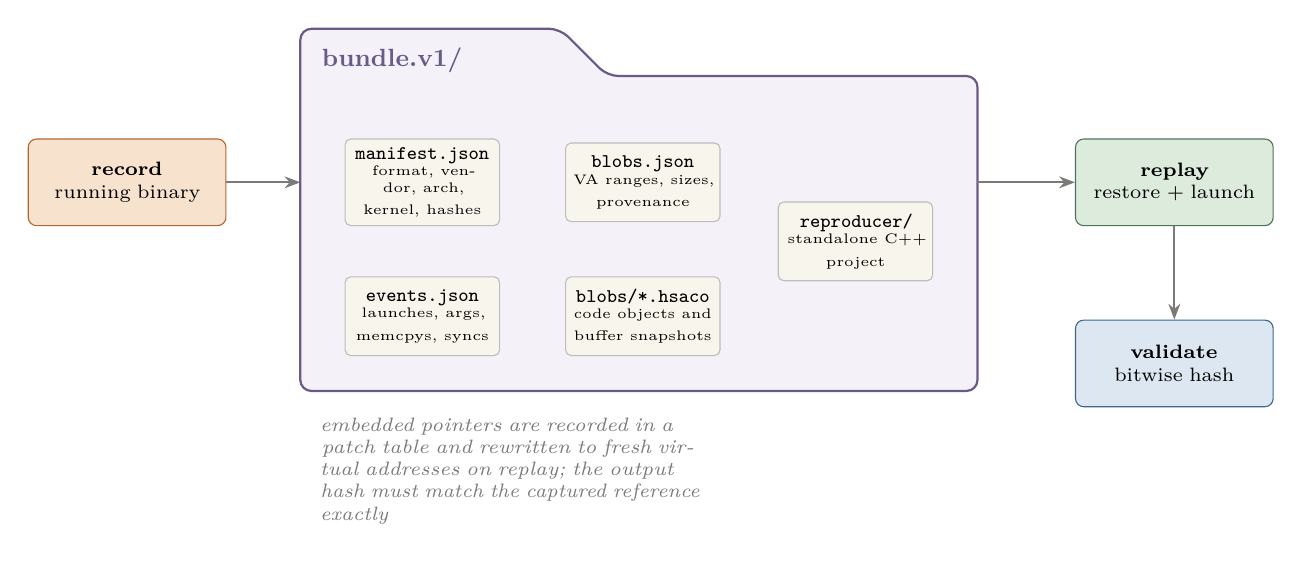
\begin{tikzpicture}[
    font=\small,
    stage/.style={draw, rounded corners=3pt, align=center, text width=2.3cm,
                  minimum height=1.1cm, inner sep=3pt, font=\scriptsize, fill=paper},
    part/.style={draw=ink!30, rounded corners=2pt, align=center, text width=1.75cm,
                 minimum height=1.0cm, inner sep=3pt, font=\scriptsize, fill=ink!3},
    flow/.style={-{Stealth[length=2mm]}, line width=0.8pt, draw=ink!60},
    note/.style={font=\scriptsize\itshape, text=ink!60, align=left},
  ]

  % The bundle folder.
  \draw[draw=kviolet, fill=kvioletfill!45, rounded corners=4pt, line width=0.8pt]
    (0.2,-1.9) -- (8.8,-1.9) -- (8.8,2.1) -- (4.1,2.1) -- (3.5,2.7) -- (0.2,2.7) -- cycle;
  \node[font=\small\bfseries, text=kviolet, anchor=west] at (0.35,2.3) {bundle.v1/};

  \node[part, fill=paper] (man) at (1.75,0.75)
    {\texttt{manifest.json}\\{\tiny format, vendor, arch,\\kernel, hashes}};
  \node[part, fill=paper] (events) at (1.75,-0.95)
    {\texttt{events.json}\\{\tiny launches, args,\\memcpys, syncs}};
  \node[part, fill=paper] (blobs) at (4.55,0.75)
    {\texttt{blobs.json}\\{\tiny VA ranges, sizes,\\provenance}};
  \node[part, fill=paper] (snap) at (4.55,-0.95)
    {\texttt{blobs/*.hsaco}\\{\tiny code objects and\\buffer snapshots}};
  \node[part, fill=paper] (repro) at (7.25,0.0)
    {\texttt{reproducer/}\\{\tiny standalone C++\\project}};

  % Record and replay around the folder.
  \node[stage, fill=korangefill, draw=korange] (record) at (-2.0,0.75)
    {\textbf{record}\\running binary};
  \node[stage, fill=kgreenfill, draw=kgreen] (replay) at (11.3,0.75)
    {\textbf{replay}\\restore + launch};
  \node[stage, fill=kbluefill, draw=kblue] (check) at (11.3,-1.55)
    {\textbf{validate}\\bitwise hash};
  \draw[flow] (record) -- (0.2,0.75);
  \draw[flow] (8.8,0.75) -- (replay);
  \draw[flow] (replay) -- (check);
  % The patch table is the subtle part of VA fidelity.
  \node[note, anchor=north west, text width=4.8cm] at (0.35,-2.12)
    {embedded pointers are recorded in a patch table and rewritten to fresh
     virtual addresses on replay; the output hash must match the captured
     reference exactly};
\end{tikzpicture}
}
\caption{Bundle v1. The manifest names the vendor and mechanism; the event log
records API calls, allocations, launches, copies, memsets, streams, modules,
and parameter metadata; the blob index carries a SHA-256 and a patch table for
every snapshot.}
\label{fig:capture}
\end{figure}

A v1 bundle is a directory:
\begin{lstlisting}
<name>.kcap/
  manifest.json
  events.json
  blobs.json
  blobs/b0001.bin
\end{lstlisting}

\kst{manifest.json} must have \kst{format_id="kernscope-capture"},
\kst{schema_version="1.0"}, \kst{vendor} in \{nvidia, amd, mock\},
\kst{capture_mechanism} in \{cupti, preload, hip-sdk\},
\kst{snapshot_policy="va-faithful"}, and a \kst{size_governance} object with a
default maximum snapshot of 1\,GiB. A total over the cap stops further blob
writes, sets \kst{aborted=true}, records a reason, and leaves a loadable
partial bundle.

\kst{events.json} is an ordered log. The record types are API counts,
allocation and free, unknown free, launch, copy, memset, stream, fatbin,
cubin, and parameter info. A launch carries the kernel name, the launch
mechanism, grid/block/shared memory, stream and graph handles, and a
per-parameter argument table. Each argument is a pointer or scalar, with a
size, a byte-exact host copy, and the original virtual address for pointer
slots.

\kst{blobs.json} indexes the snapshots. Each blob has an id, file, role, VA,
size, SHA-256, and patch table. Roles are kernel binary, input, output,
argument, and state. The reader recomputes every hash on read and rejects a
mismatch. The patch table is the mechanism that makes replay portable: every
8-byte little-endian value in a blob that equals a known allocation VA is
recorded as a patch, and replay rewrites only the entries present in the
allocation remap. A \kst{__device__} global that happens to contain another
global's address is out of scope.

\subsection{Replay, validation, and benchmark}
\label{sec:c4-replay}

The replay model resolves buffers from allocations, H2D inputs, D2H markers,
and v1 snapshots, then restores the binary, the argument plan, and the launch
geometry. HIP/HSA assigns virtual addresses, and the current runtime wrapper
does not expose CUDA VMM placement, so replay remaps on both vendors. It
allocates fresh buffers, computes old-to-new VA remapping, applies the patch
tables before upload, rewrites pointer argument slots through the same table,
and launches the captured grid, block, and shared memory.

Validation is bitwise by default: byte compare plus SHA-256, with a hash diff
on failure. Tolerance mode interprets outputs as bf16 chunks upcast to fp32
and passes only when cosine $\ge 0.999$, maximum relative error
$\le 10^{-2}$, and PCC $\ge 0.99$. References come from v1 output snapshots
or from \kst{--ref} in output-buffer order; a missing reference is an error,
not a pass.

\kst{bench} performs one validation launch before timing and refuses to time
an invalid replay unless \kst{--no-validate} is given. It uses ten repetitions
by default, an L2 flush, event timing, and median plus p20/p80. Each run
writes one \kst{libs/db} record keyed by architecture and kernel hash, with
\kst{provenance.mode="measured"}.

\subsection{Reproducer and size governance}
\label{sec:c4-repro}

\kst{emit-repro} writes a standalone plain-CMake C++ project with the kernel
binary, inputs, a \kst{main.hip} or \kst{main.cu}, a \kst{CMakeLists.txt}
pinned to the manifest vendor and architecture, and a README. It re-points
pointer arguments at fresh buffers and launches the captured geometry.
Size-unknown buffers become deterministic synthetic inputs, marked so a reader
does not mistake them for bit-exact data. The NVIDIA reproducer is
compile-only.

\subsection{CUDA/HIP field mapping}
\label{sec:c4-mapping}

The mapping contract compares what the two vendors can both express, after
normalization. Kernel names are compared after stripping the \kst{.kd} suffix
and demangling. Grid, block, and shared memory compare directly. The default
stream normalizes to 0; non-default streams get a 1-based id. Pointers compare
as 1-based allocation ordinals, not raw VAs. Scalars compare by size and
byte-identical value; input blobs compare by SHA-256 after H2D call order.
Allocations compare as a sorted multiset of sizes; copies compare by kind
(H2D, D2H, D2D). Binary blobs are compared per vendor only; a cubin is never
compared with an hsaco. API counts, raw pointers before normalization, and
timestamps are not compared.

\subsection{Measured evidence}
\label{sec:c4-evidence}

The demo captured the hot layernorm kernel
\kst{_Z15layernorm_fused}\allowbreak\kst{PKtS0_S0_Ptfi.kd} into a v0
text bundle. The v1 layout is the current reader contract and the
capture-tune path accepts it, but the record CLI in this tree still writes
the v0 form; the gap is flagged in \Cref{sec:limitations-list}. The launch
was at grid
$1024 \times 1 \times 1$ and block $128 \times 1 \times 1$. The bundle has
three blobs. Replay reproduced the output bitwise; the reference SHA-256 is
\kst{a0027ed9a8ef2e3453aeb194aa64108c}\allowbreak\kst{1f300a87fbfa292cca5222a725449eec}.
The capture-tune stage then explored four block sizes over the same bundle,
validated all four bitwise, and selected block 256. This is the strongest
cross-tool evidence in the report: the analyzer's stage-3 findings and the
tuner's stage-4 candidates both refer to the same captured code object and
launch.

% ===========================================================================
\section{C5: LLVM passes}
\label{sec:c5}

\kst{kernscope-pass} is an out-of-tree LLVM 21 pass plugin. It is loaded by
both driver paths, \kst{opt -load-pass-plugin} and
\kst{clang -fpass-plugin}, and it uses the New Pass Manager's
\kst{PassPluginLibraryInfo} entry point. The \kst{kernscope-pass-report} CLI
runs a fixed showcase pipeline and measures the before/after delta with the
analyzer.

\subsection{Plugin structure}
\label{sec:c5-plugin}

A pass module subclasses \kst{llvm::}\allowbreak\kst{PassInfoMixin} and
registers a callback with \kst{REGISTER_PASS_}\allowbreak\kst{CALLBACK} at
file scope. The callback receives the
\kst{PassBuilder} of the loading process and wires the module into the
pipeline. The registry is a process-global singleton; the plugin entry point
does not need to know the module names in advance. The lit suite exercises
both \kst{opt} and \kst{clang} loading so an ABI change fails at the loader
rather than at the first transformed kernel.

\subsection{The passes}
\label{sec:c5-passes}

\begin{table}[htbp]
\centering
\small
\begin{tabularx}{\textwidth}{@{}l@{\hspace{1em}}X@{}}
\toprule
Pass & Transformation or analysis \\
\midrule
\kst{kernscope-promote} & Global-to-shared promotion for tiles reused in a loop. \\
\kst{kernscope-tile} & Loop tiling over constant-trip, unit-stride \kst{\{s,+,1\}} windows. \\
\kst{kernscope-vectorize} & Rewrites scalar load/store chains into vector operations when alignment and contiguity permit. \\
\kst{kernscope-pad} & Shared-memory padding to break a known bank-conflict stride. \\
\kst{kernscope-rle} & Redundant-load elimination and address simplification. \\
\kst{kernscope-coalesce} & Analysis of per-access coalescing class; no rewrite. \\
\bottomrule
\end{tabularx}
\caption{The pass modules. The coalescing analysis is shared with the
analyzer's 128-byte-sector model so before/after numbers use the same
definition.}
\label{tab:c5passes}
\end{table}

The default showcase pipeline is
\kst{kernscope-tile},\allowbreak
\kst{kernscope-promote},\allowbreak
\kst{kernscope-vectorize},\allowbreak
\kst{kernscope-pad},\allowbreak
\kst{kernscope-coalesce}.
Not every pass fires on every kernel; a no-transform result is a valid
outcome and is recorded as such. The tile pass, for example, declines a
layernorm loop whose induction variable is not a canonical \kst{\{0,+,1\}}
phi.

\subsection{The delta report}
\label{sec:c5-delta}

\kst{kernscope-pass-report --report-pipeline <gemm|layernorm|softmax>} runs
clang to before-IR, the plugin pipeline to after-IR, and \kst{llc} to
before/after PTX. It then invokes \kst{kernscope-analyze} on both PTX files
and emits a delta report with register estimate, shared-memory bytes,
coalescing class, bank-conflict way, vector width, and vectorized global
loads. Every metric is labeled improved, unchanged, or not applicable. The
report's provenance is \kst{projected}: the IR and PTX are compile-only
artifacts, and the note says the measured gfx1101 analog lives in the
\kst{libs/db} records.

On layernorm, vector width goes from 1 to 4, vectorized global loads from 0 to
12, uncoalesced accesses from 64 to 16, and the register estimate stays at
175. The pass report records 12 vector chains and 48 vectorized loads. gemm
and softmax are correctly left no-transform, and all three kernels compile to
PTX with exit 0 after the pipeline. The tile pass's refusal is recorded with
its reason rather than hidden.

% ===========================================================================
\section{C6: profiler}
\label{sec:c6}

\kst{kernscope-profile} answers three questions from a running binary: which
kernels ran, how long each took, and what the compiler-visible facts suggest
about the bottleneck. It does not require hardware counters. It traces, it
enriches, it ranks, and it diagnoses from the activity records and the
architecture database.

\subsection{Pipeline}
\label{sec:c6-pipeline}

\begin{enumerate}
  \item \textbf{Trace.} The target runs under \kst{LD_PRELOAD} of the
        rocprofiler-sdk tracer; each kernel dispatch and HIP API call becomes a
        JSONL record. On NVIDIA the equivalent path is the CUPTI activity
        tracer, which is compile- and unit-tested locally and rental-gated for
        live use.
  \item \textbf{Enrich.} Each kernel record receives occupancy and limiter
        estimates from \fpath{libs/occupancy}, code-object VGPR/SGPR/LDS
        facts where available, and explicit degradation markers where not.
  \item \textbf{Rank.} Kernels are grouped by name and ranked by total time
        (then median, then name); the top ten are kept.
  \item \textbf{Diagnose.} The rule engine classifies memory, latency, and
        compute behavior for known families, reports the occupancy limiter,
        and degrades to \kst{insufficient_evidence} rather than inventing a
        cause.
  \item \textbf{Report.} \kst{--json} emits the model, \kst{--text} the
        owner-facing table, and \kst{--html} a self-contained page with the
        embedded JSON.
\end{enumerate}

\subsection{Diagnostics}
\label{sec:c6-diagnostics}

A \kst{memory_bound} hint is emitted when the workload's arithmetic intensity
is below the measured ridge point. A \kst{latency_bound} or
\kst{compute_bound} hint follows the same roofline position and the
instruction mix. An occupancy limiter hint is emitted when occupancy is below
1.0; the limiter is the binding resource. Sub-hints distinguish register
bloat, shared-memory pressure, and a block too small to fill the machine.
Every hint carries its evidence: arithmetic intensity, bytes moved, ridge
point, occupancy, registers, or the analyzer finding id when the analyzer was
merged into the pipeline.

\subsection{Measured evidence}
\label{sec:c6-evidence}

Tracing the layernorm app produced three kernels and 19.6\,$\mu$s of wall
time. The hot kernel ran for 9.2\,$\mu$s with 24 registers per thread,
occupancy 1 (limiter registers), 1024 bytes of shared memory, grid
$1024 \times 1 \times 1$, and block $128 \times 1 \times 1$. The profiler
emitted a memory-bound hint with arithmetic intensity 1.375, a bytes-moved
estimate of 1048576, and a ridge point of 27.614. The hint's
\kst{analyzer_cross_refs} in the aggregated report point at the stage-3
analyzer findings, including \kst{possibly_divergent_branch}.

% ===========================================================================
\section{Bench, dashboard, and the evidence layer}
\label{sec:dashboard}

\subsection{Benchmark methodology}
\label{sec:bench-method}

\kst{libs/bench} is the one timing method in the project. It warms up the
kernel, flushes L2 between trials, and adapts the trial count to a time budget
while keeping a minimum sample count. It reports the median and the p20/p80
quantiles, not a mean, so a single slow launch does not move the result. The
same harness times the peak microbenchmarks, the tuner variants, and the
capture-replay benchmark. A correctness gate runs before timing in the
tuner and in capture replay; the peak microbenchmarks are their own reference.

\subsection{Measured machine peaks}
\label{sec:peaks}

The peaks in \Cref{tab:peaks} drive the roofline engine. The fp32 figure is
the register-resident FFMA loop; the DRAM read figure uses a 512\,MiB array;
the LDS figure is a read-plus-write loop. The device-to-device figure is
reported as a range over the accepted runs. Clocks were recorded with
\kst{rocm-smi} but not locked, and the machine was not isolated from
development activity. The numbers are therefore a measured description of
this machine on 2026-08-14, not a datasheet claim.

\subsection{Dashboard sections}
\label{sec:dashboard-sections}

The dashboard aggregates six sections. Each section has a title, an
availability flag, a status, a provenance object, a summary, and a list of
evidence paths.

\begin{table}[htbp]
\centering
\small
\begin{tabularx}{\textwidth}{@{}l l X@{}}
\toprule
Section & Mode & Summary at consolidation \\
\midrule
\kst{analyzer} & projected & Golden occupancy 0.375, 102 registers, limiter registers, 3 warnings, 3 suggestions. \\
\kst{tune} & measured & 15 matmul variants; best 415.324\,$\mu$s, worst 3.106\,ms. \\
\kst{verify} & projected & 34 entries, 19 files, 8 classes; 18 SAFE. \\
\kst{capture} & measured & Grid $1024\times1\times1$, block $128\times1\times1$, 3 blobs, bitwise PASS. \\
\kst{profile} & measured & 3 kernels, 19.6\,$\mu$s wall, hot 9.2\,$\mu$s, memory-bound hint. \\
\kst{pass} & projected & Layernorm vector width 1$\rightarrow$4, uncoalesced 64$\rightarrow$16; gemm/softmax no-transform. \\
\bottomrule
\end{tabularx}
\caption{Dashboard sections and their provenance modes. The mode is a
convention recorded by the aggregator; the report schema does not require it.}
\label{tab:dashboard}
\end{table}

\subsection{What the provenance does and does not enforce}
\label{sec:provenance}

The report schema (\Cref{app:report-schema}) requires \kst{kernel},
\kst{metrics}, \kst{limiter}, \kst{warnings}, and \kst{suggestions}. It does
not require \kst{schema_version} or \kst{provenance}; those are report-engine
and dashboard conventions. The per-section provenance object has a
\kst{mode} in \{measured, projected, no\_data\} and a boolean
\kst{measured}. The dashboard validator asserts the six sections, the boolean,
the evidence files, and the rendered module markers. The validator is not
called by \kst{ci.sh}; it is a separate check. The report states this because
a provenance convention that is described as enforced when it is only
intended is exactly the kind of claim this project is trying to avoid.

% ===========================================================================

% ===========================================================================
\clearpage
\floraon
\florathispage{layout=surround, seed=41, density=0.32, visitors=0.08}
\part{Evidence and operation}
\thispagestyle{empty}
\clearpage
\floraoff
% ===========================================================================

\section{Testing, CI, and reproducibility}
\label{sec:repro}

\subsection{The four test layers}
\label{sec:test-layers}

The gate is layered so a regression stops at the cheapest test that can see
it:
\begin{enumerate}
  \item \textbf{gtest / ctest.} C++ unit and integration tests carry one
        hardware label: \kst{no-gpu}, \kst{gpu-amd}, or
        \kst{gpu-nvidia-rental}. The first two are the local gate; the third is
        owner-executed on a rental.
  \item \textbf{lit / FileCheck.} The \kst{check-kernscope} target runs the
        parser, pass, verifier-manifest, and CLI tests against committed IR and
        ISA corpora.
  \item \textbf{NumPy bf16 golden harness.} \kst{pytest tests/golden} compares
        generated kernels against reference outputs under the bf16 tolerance
        contract. It is the independent implementation of the C++ golden gate.
  \item \textbf{Generated-code compile checks.} \kst{scripts/compile_checks.sh}
        compiles the template variants with \kst{nvcc} for sm\_80/sm\_90
        (compile-only) and \kst{hipcc} for gfx1101, then runs the live HIP
        variant through the golden gate.
\end{enumerate}

\subsection{The CI gate}
\label{sec:ci}

\kst{scripts/ci.sh} runs the stages in order and exits non-zero on the first
failure. A stage whose artifact is absent prints \kst{[SKIP]} and stays green,
which is a bootstrap convenience, not a claim that the stage ran.

\begin{table}[htbp]
\centering
\small
\begin{tabularx}{\textwidth}{@{}l X@{}}
\toprule
Stage & Check \\
\midrule
a & \kst{scripts/configure.sh} and \kst{cmake --build build}. \\
b & \kst{ctest -L "no-gpu|gpu-amd"} with hardware labels. \\
b2 & Non-decreasing count guard against \kst{scripts/ci-baseline.txt} (550). \\
c & \kst{cmake --build build --target check-kernscope} (lit/FileCheck). \\
d & \kst{pytest tests/golden -q} (NumPy bf16 goldens). \\
e & \kst{scripts/compile_checks.sh} (nvcc sm\_80/90, hipcc gfx1101, live HIP golden). \\
f & Committed fixtures total at most 64\,MB (\kst{du -sm tests/fixtures}). \\
g & NVIDIA-header guards: no vendored CUDA/CUPTI/NVTX header filenames or vendor copyright markers outside the documented exceptions. \\
\bottomrule
\end{tabularx}
\caption{The CI stages. The count guard is non-decreasing, not exact: adding
tests is always green, and removing a registration below the floor fails.}
\label{tab:ci}
\end{table}

The \kst{CI_SKIP_CONFIGURE=1} escape hatch skips configure and build. It exists
for a bootstrap situation where the nix-store LLVM resolution is being
repaired; it is owner-set and it makes the skip visible. The gate does not run
the dashboard validator, and it does not run a secret scanner. Those are
operational gaps, not hidden passes.

\subsection{The master reproducibility script}
\label{sec:reproduce-all}

\kst{scripts/reproduce-all.sh} chains four stages: the lock check,
\kst{ci.sh}, \kst{demo.sh}, and the dashboard. The lock check requires
\kst{devenv.lock} to exist and be tracked; it never regenerates the lock
silently. The dashboard writes \fpath{reports/dashboard.html} and
\fpath{reports/dashboard.json} with \kst{SOURCE_DATE_EPOCH} defaulted to the
HEAD commit time, so two runs on the same commit can be byte-identical.

A clean checkout is:
\begin{lstlisting}
devenv shell
git clone https://github.com/meillaya/kernscope.git
cd kernscope
bash scripts/ci.sh
bash scripts/reproduce-all.sh
\end{lstlisting}
The first configure and build are the slowest (roughly ten minutes on the
reference machine); later runs reuse \fpath{build/}. The committed fixtures,
golden inputs, lit corpora, and schema files are the complete gate input. The
earlier documentation used a local absolute clone path; this report states the
public URL instead.

\subsection{Owner-gated NVIDIA runs}
\label{sec:rental-runbook}

Only \kst{scripts/rental-validate.sh} runs NVIDIA code. It is never called by
\kst{ci.sh}. In \kst{--dry-run} it prints the sequence: SSH to the rental host,
check \kst{nvcc}, detect the CUPTI version from \kst{cupti_version.h}, run
\kst{ctest -L gpu-nvidia-rental}, and place evidence under
\fpath{reports/rentals/}. In exec mode it refuses when \kst{CI=true}, requires
a configured build tree, probes \kst{$CUDA_HOME}, \fpath{/usr/local/cuda}, and
\fpath{/opt/cuda} for CUPTI, and writes a timestamped summary with the verdict,
exit code, CUDA major, and CUPTI version.

The gate is procedural. The script checks the environment, not the operator's
identity, and it assumes SSH keys are already configured. The repository
ignores \fpath{reports/rentals/*} except the placeholder, so an owner who wants
to commit a rental summary must force-add it. No rental numbers are claimed in
this report.

\subsection{Secrets and sensitive data}
\label{sec:secrets}

The repository ignores \fpath{private_key.pem}, \fpath{public_key.pem},
\fpath{.env}, and \fpath{.env.*} (with an exception for \fpath{.env.example}).
The rental script does not manage keys. There is no secret scan in \kst{ci.sh};
the rule is enforced by the ignore list and by review, not by an automated
gate. Capture bundles are local-only and gitignored; snapshot sizes are capped
at 1\,GiB by default, and the fixture budget is 64\,MB.

% ===========================================================================
\section{Evaluation}
\label{sec:eval}

\subsection{The demo run}
\label{sec:eval-demo}

\kst{scripts/demo.sh} ran the loop on the local gfx1101 in 153\,s against a
900\,s budget. The aggregated report is the primary cross-tool evidence.

\begin{table}[htbp]
\centering
\small
\begin{tabularx}{\textwidth}{@{}l l X@{}}
\toprule
Stage & Status & Evidence \\
\midrule
1 profile & ok & 3 kernels, 19.6\,$\mu$s wall, hot layernorm 9.2\,$\mu$s, 24 registers, occupancy 1, \kst{memory_bound} hint (AI 1.375, ridge 27.614). \\
2 capture & ok & Bundle \fpath{bundle.v0}, 3 blobs, grid $1024\times1\times1$, block $128\times1\times1$, bitwise replay PASS, reference SHA-256 \kst{a0027e...49eec}. \\
3 analyze & ok & Captured AMDGPU ISA, 216 ALU ops, \kst{possibly_divergent_branch} warning, three informational findings. \\
4 capture-tune & ok & 4 candidates validated, baseline block 128 at 0.01208\,ms, best block 256 at 0.01206\,ms, speedup $1.0017\times$. \\
5 verify + pass & ok & 13 bias\_gelu variants, 12 compiled, 1 gated; best 0.17184\,ms vs 0.20332\,ms, $1.1832\times$; pass vector width 1$\rightarrow$4, loads 0$\rightarrow$12, uncoalesced 64$\rightarrow$16. \\
\bottomrule
\end{tabularx}
\caption{The five demo stages. The report's cross-tool block links the stage-3
analyzer finding ids to the stage-1 profiler hint.}
\label{tab:demo}
\end{table}

The cross-tool link is the part that matters. The profiler's
\kst{memory_bound} hint carries \kst{analyzer_cross_refs} with the finding ids
\kst{possibly_divergent_branch}, \kst{no_tensor_core_usage},
\kst{occupancy_not_applicable}, and \kst{suggestions_not_applicable}, and the
stage-3 evidence path. The analyzer ran on the captured kernel's
disassembled ISA, not on a hand-picked example. The verifier removed one
variant before compilation. The pass delta used the analyzer's own metrics.
This is the concrete meaning of ``the loop closes'' in this report.

\subsection{Analyzer and verifier evidence}
\label{sec:eval-static}

The analyzer golden fixture is described in \Cref{sec:c1-evidence}. The
verifier corpus has 34 entries across 19 source files, with 18 \kst{SAFE}
verdicts and 16 non-\kst{SAFE} verdicts spread across the bounds, race,
barrier, pointer, uninitialized-read, and address-space classes. Both results
are \kst{projected}: they come from static analysis, not from a GPU run. The
verifier's anti-self-report gate diffs the CLI's JSON against the manifest read
from disk, so a corrupted expectation fails the lit suite.

\subsection{Tuner and capture evidence}
\label{sec:eval-live}

The capture-tune and verify-tune results in \Cref{tab:demo} are measured on
gfx1101. The capture path is bitwise: every explored config must reproduce the
captured output hash before it is timed. The template path is
correctness-gated: a variant that fails cosine, relative error, or PCC is
discarded, not timed. The measured speedups are small for capture-tune
(1.0017$\times$) and modest for the bias\_gelu template search
(1.1832$\times$); the report quotes them as measured, not as a general
speedup claim.

The dashboard records a separate matmul search with 15 measured variants and a
best median of 415.324\,$\mu$s. The raw JSONL for that run is not committed,
so this is a dashboard-sourced value, not a value reconstructed from a raw
record. The distinction matters because the dashboard's tune section lists
source paths that are absent from the tree.

\subsection{Pass and profile evidence}
\label{sec:eval-projected}

The layernorm pass delta is projected: vector width 1$\rightarrow$4,
vectorized global loads 0$\rightarrow$12, uncoalesced accesses
64$\rightarrow$16, registers unchanged at 175. The before/after PTX compiles
cleanly, and gemm and softmax are correctly no-transform. The report does not
claim a wall-clock pass speedup; it claims the static delta that the pipeline
measures.

The profiler evidence is measured: 3 kernels, 19.6\,$\mu$s wall, a
9.2\,$\mu$s hot kernel, 24 registers, occupancy 1, and a memory-bound hint
with arithmetic intensity 1.375 and ridge point 27.614. The hint is a
compiler-aware diagnosis from activity records and the roofline, not from
hardware counters.

\subsection{Threats to validity}
\label{sec:threats}

\begin{itemize}
  \item \textbf{One measured platform.} Every live number is gfx1101 on one
        RX 7800 XT. The same kernel on CDNA or NVIDIA may behave differently.
  \item \textbf{Unlocked clocks.} The peak run recorded clocks with
        \kst{rocm-smi} but did not lock them, and the machine was shared with
        development activity. The peaks are a description of this machine at
        that time.
  \item \textbf{Projected deltas.} The pass numbers are static IR/PTX
        artifacts. They are not wall-clock speedups.
  \item \textbf{Verifier scope.} The verifier is a may-analysis, not a formal
        prover. Its false-positive and false-negative classes are stated in
        \Cref{sec:c3-soundness}.
  \item \textbf{Dashboard gaps.} The tune section's source files are absent;
        the matmul number is quoted from the dashboard, and the validator is
        not part of \kst{ci.sh}. The report says so rather than presenting the
        dashboard as a complete raw archive.
  \item \textbf{Documentation consolidation.} The raw Markdown notes and the
        committed JSON/HTML evidence were folded into this report and removed
        from the tree. The values remain; the raw files do not. Regeneration is
        possible with the committed scripts on a gfx1101 machine.
\end{itemize}

% ===========================================================================
\section{Context and prior art}
\label{sec:prior}

kernscope is an engineering synthesis, not a new verification calculus. Its
design choices follow a body of work that the project's research briefs
survey; this section states the main lineages and what kernscope borrows or
declines.

\subsection{Performance models and static analysis}
\label{sec:prior-analysis}

The roofline model \citep{roofline2009} supplies the compute and memory
ceilings and the ridge point used by the tuner and profiler. Occupancy follows
the CUDA programming guide's resource model \citep{cudaProgrammingGuide}, with
the low-occupancy/high-ILP trade-off documented by Volkov
\citep{volkov2010}. Nsight Compute's Speed of Light vocabulary
\citep{nsightComputeSOL} is the diagnostic register the profiler adopts.

The analyzer's static estimates sit against a line of microbenchmark-driven
architecture studies (Volta, Turing, Hopper, and CDNA3) and against simulators
such as GPGPU-Sim and Accel-Sim \citep{gpgpusim2009,accelsim2020} and binary
instrumentation such as NVBit \citep{nvbit2019}. Those tools measure or
simulate; kernscope reads the ISA text and the architecture database, which is
cheaper and less precise. The analyzer's contribution is the reuse of the same
architecture constants and metrics by the tuner, pass report, and profiler.

\subsection{Autotuning and tensor compilation}
\label{sec:prior-tune}

The autotuner follows the algorithm/schedule separation of Halide
\citep{halide2013}, the search-based scheduling of TVM and Ansor
\citep{tvm2018,ansor2020}, and the tile-level autotuning model of Triton
\citep{triton2019}. CUTLASS \citep{cutlass} and the vendor libraries set the
performance bar; Kernel Tuner \citep{kerneltuner2024} is the closest standalone
autotuner prior art. FlashAttention \citep{flashattention2022} motivates the
memory-bound attention family and the IO-aware tiling direction. kernscope
does not generate a general tensor program; it generates family-specific
templates, gates them on correctness, and records the search in a cache that
can be replayed.

\subsection{GPU verification}
\label{sec:prior-verify}

GPUVerify \citep{gpuverify2012,gpuverify2015} is the methodological anchor:
the two-thread reduction turns race and divergence checks into sequential
program verification. PUG, SESA, GKLEE, and ESBMC-GPU
\citep{pug2010,sesa2014,gklee2012,esbmcgpu2017} explore symbolic execution and
bounded model checking. Faial \citep{faial2024} contributes behavioral types
over index expressions and the finding that most data-race-free kernels need a
thread-configuration assumption. HiRace and HGRD
\citep{hirace2024,hgrd2026} bring dynamic and MLIR-level analyses. LLOV
\citep{llov2020} demonstrates static race freedom on LLVM IR. The Linux eBPF
verifier \citep{ebpfVerifier} supplies the interaction model: typed ranges,
bounded state exploration, and a concrete rejection reason. MemorySanitizer
\citep{msan2015} and the SPIR-V validator \citep{spirvSpec} inform the
uninitialized-read and well-formedness checks.

kernscope-verify is deliberately smaller: eight may-analyses over LLVM IR at
\kst{-O1}, with the launch configuration ingested from the host half and a
three-tier exact/upper-bound/symbolic contract. It does not claim the
soundness of GPUVerify or Faial, and its false-positive and false-negative
classes are published rather than hidden.

\subsection{Capture and replay}
\label{sec:prior-capture}

Kerncap \citep{kerncap2026} is the closest complete system: HSA-level
extraction and VA-faithful replay for HIP and Triton. Mneme \citep{mneme2023}
records and replays kernels for tuning; the LLNL Record-Remix-Replay line
\citep{r3-2026} and Tally \citep{tally2024} explore the same design space.
CUPTI \citep{cupti} and rocprofiler-sdk \citep{rocprofilerSDK} provide the
vendor tracing surfaces. kernscope's contribution is the shared bundle model
across CUPTI, LD\_PRELOAD, and rocprofiler-sdk, the explicit patch table for
embedded pointers, and the use of the same bundle by the analyzer,
capture-tune, and the standalone reproducer.

\subsection{LLVM passes and profiling}
\label{sec:prior-pass}

The pass plugin uses LLVM's New Pass Manager and the out-of-tree
\kst{PassPluginLibraryInfo} ABI \citep{llvm2004,mlirCGO2021}. The
transformations are deliberately narrow: promotion, tiling, vectorization,
padding, redundant-load elimination, and a coalescing analysis. The GPU
backends already run address-space inference, load/store vectorization, and
redundant-load elimination; the project's value is the analyzer-measured
before/after delta, not a claim that these transformations are new. IREE
\citep{iree} is the closest production analog for a compiler-integrated
memory-optimization pipeline.

The profiler follows the activity-only tier of CUPTI and rocprofiler-sdk plus
the roofline and occupancy vocabulary of Nsight Compute
\citep{nsightComputeSOL}. It reports what it can evidence and degrades to
\kst{insufficient_evidence} when the family, PTX, or occupancy is unknown.

% ===========================================================================
\section{Limitations and future work}
\label{sec:limits}

\subsection{Limitations}
\label{sec:limitations-list}

\begin{itemize}
  \item \textbf{No NVIDIA runtime evidence.} CUPTI capture, CUPTI profiling,
        and NVIDIA runtime benchmarks are compile- and unit-tested only. The
        rental path exists but produced no committed numbers.
  \item \textbf{One measured GPU.} The measured results are gfx1101 only. The
        analyzer supports other architectures, but their occupancy and
        roofline numbers are not validated here.
  \item \textbf{Pass deltas are projected.} The vector-width and coalescing
        improvements are static IR/PTX measurements. A wall-clock speedup for
        the transformed layernorm is not claimed.
  \item \textbf{The verifier is a may-analysis.} Data-dependent indices and
        runtime allocations degrade to non-\kst{SAFE} verdicts; atomics,
        warp-synchronous code, and inter-block races are out of scope.
  \item \textbf{Capture format drift.} The v1 schema is the reading contract,
        but the demo bundle is v0 and the current record path still uses the
        v0 environment-variable flow. The v1 writer path is not exercised by
        the demo.
  \item \textbf{Dashboard incompleteness.} The committed dashboard's tune
        section cites per-run JSONL files that are absent, and the dashboard
        validator is not invoked by \kst{ci.sh}. The matmul number is quoted
        from the dashboard only.
  \item \textbf{Report schema does not enforce provenance.} The schema
        requires the kernel, metrics, limiter, warnings, and suggestions; the
        provenance object is a report-engine and dashboard convention.
  \item \textbf{Tooling gaps.} The auxiliary PTX dump source has no CMake
        target and is not built. The capture CLI's usage exit codes do not
        consistently match the documentation. The report names these rather
        than presenting a uniform interface that does not exist.
  \item \textbf{The archive is textual.} The consolidation removed the raw
        JSON/HTML evidence. The numbers in this report are preserved, but a
        reader who needs the raw records must regenerate them on a gfx1101
        machine with the committed scripts.
\end{itemize}

\subsection{Future work}
\label{sec:future}

\begin{enumerate}
  \item \textbf{Run the NVIDIA rental.} Execute \kst{rental-validate.sh} on an
        A100/H100 host, commit the summary with the same provenance schema, and
        add an NVIDIA column to the dashboard.
  \item \textbf{Exercise CUDA 13.} Build the record adapter against
        \kst{CUPTI_API_VERSION} 130001 and turn the Kernel9/Kernel10
        \kst{static_assert}s into a tested migration.
  \item \textbf{Close the v0/v1 capture gap.} Make \kst{record} write the v1
        bundle by default, exercise the schema in the demo, and remove the
        environment-variable path.
  \item \textbf{Strengthen the verifier.} Add HGRD-style barrier intervals,
        Faial-style index types, and a PTX well-formedness layer; keep the
        false-positive and false-negative tables current.
  \item \textbf{Wire evidence into CI.} Run the dashboard validator in
        \kst{ci.sh}, fix its failure path, and add a secret scan.
  \item \textbf{Roofline-driven pass selection.} Choose vectorization or tiling
        from the profiler's bound class and the pass report's predicted delta,
        then validate the choice with a measured benchmark.
  \item \textbf{Validate generated kernels.} Use the verifier and golden gate
        as a correctness harness for LLM-generated CUDA, with a kernel-benchmark
        sweep rather than a single family.
\end{enumerate}

% ===========================================================================
\section{Conclusion}
\label{sec:conclusion}

kernscope's claim is modest and testable: a GPU-kernel toolchain can share one
library stack, one report schema, and one provenance discipline, and its tools
can validate each other instead of self-reporting. The loop runs on one local
GPU in 153\,s. The analyzer reads the captured ISA, the verifier removes a
risky variant before compilation, the capture replay is bitwise, and the pass
delta is measured with the same metrics the analyzer uses. The numbers are
small where the work is small (a 1.0017$\times$ capture-tune speedup) and
larger where the search has room (a 1.1832$\times$ bias\_gelu speedup); the
report keeps them in their provenance categories.

The same discipline that makes the evidence useful makes the limits visible.
There are no NVIDIA runtime numbers, the pass deltas are projected, the
verifier is not a prover, one GPU supplied every live measurement, and the
dashboard is not a complete raw archive. Those are not caveats appended to the
claim; they are the conditions under which the claim is true. The repository's
scripts can regenerate the evidence on a gfx1101 machine, and this report is
the archival account of what was present when the documentation was
consolidated.

% ===========================================================================

% ===========================================================================
\appendix
% ===========================================================================

\section{CLI reference}
\label{app:cli}

\begin{longtable}{@{}p{3.6cm}p{10.7cm}@{}}
\toprule
Tool & Synopsis and notable options \\
\midrule
\endhead
\kst{kernscope-analyze} &
\kst{<file.ptx|file.s|file.isa> [--arch A] [--block N] [--json|--text|--html]
[--source F] [--version] [--help]}. Exit 0 clean, 1 warnings, 2 parse/arch/
schema error, 3 usage. \\
\addlinespace
\kst{kernscope-tune} &
\kst{--kernel F --shape S --arch A [--grid auto|full] [--json|--html|--text]
[--db P] [--cache P] [--workdir D] [--min-occupancy X] [--no-bench]
[--no-cache|--force] [--emit-repro D] [--verify] [--inject-risky F]
[--gate-shape S] [--version] [--help]}. Exit 0 best selected, 1 no viable
config, 2 usage/environment, 3 unknown family. \\
\addlinespace
\kst{kernscope-tune} &
\kst{--from-capture B [--vendor amd] [--arch gfx1101] [--blob-dir D]
[--kernel K] [--ref F] [--candidates CSV] [--inject-config C] [--reps N]
[--no-flush] [--db P] [--profile-out P] [--json|--text]}. Exit 0 best,
1 no valid config, 2 usage/environment. \\
\addlinespace
\kst{kernscope-verify} &
\kst{<src.cu|src.hip> [--device-only] [--json] [--out BASE] [--list-checks]
[--budget N] [--opt O1|O2] [--arch sm_80|gfx1101] [--version]}. Exit 0
approved, 1 error-class verdict, 2 ingestion failure, 3 usage. \\
\addlinespace
\kst{kernscope-capture} &
\kst{record <app> [args] [--vendor auto|amd|nvidia] [--bundle P]
[--blob-dir D] [--env K=V]} \\
& \kst{replay <bundle> [--vendor A] [--arch A] [--blob-dir D] [--kernel K]
[--mode bitwise|tolerance] [--ref F] [--dump-dir D] [--profile-out P]} \\
& \kst{bench <bundle> [replay flags] [--reps N] [--no-flush] [--no-validate]
[--db P] [--profile-out P]} \\
& \kst{emit-repro <bundle> [--out D] [--blob-dir D] [--vendor A] [--arch A]
[--kernel K] [--force]} \\
& \kst{db-query <db.jsonl> [--arch A] [--family F] [--shape S]}. Replay exit
0 pass, 1 validation failure, 2 cannot run; db-query 0 found, 1 none,
2 unreadable. \\
\addlinespace
\kst{kernscope-profile} &
\kst{<binary|dir> [--vendor auto|hip|cuda] [--json|--text|--html]
[--] [app args]}. Exit 0 report (including no kernels), 2 target/tracer/
schema failure, 3 usage. \\
\addlinespace
\kst{kernscope-pass-report} &
\kst{--report-pipeline gemm|layernorm|softmax [--build-dir D] [--workdir D]
[--json] [--out P] [--help] [--version]}. Exit 0 emitted, 2 pipeline/analyze
failure, 3 usage. \\
\addlinespace
\kst{kernscope-bench} &
\kst{[--db P] [--reps N] [--no-flush] ...}. The peak and replay harness;
default database \fpath{reports/peaks/gfx1101-bench.jsonl}. \\
\addlinespace
\kst{kernscope-dashboard} &
\kst{[--out P] [--missing SECTIONS]}. Aggregates the six module sections into
one self-contained HTML page and its JSON sibling. \\
\bottomrule
\end{longtable}

\section{Verifier verdicts and engine ids}
\label{app:verdicts}

\begin{table}[htbp]
\centering
\small
\begin{tabularx}{\textwidth}{@{}l l X@{}}
\toprule
Verdict & Class & Meaning \\
\midrule
\kst{SAFE} & approval & The checked property was proven for the analysed path. \\
\kst{MAY_OOB} & error & A bound was not proven; an access may be out of bounds. \\
\kst{SYMBOLIC_DIMS} & engine (100) & Launch dimensions are symbolic; runtime check suggested. \\
\kst{BARRIER_MISMATCH} & error & Barrier counts differ between paths. \\
\kst{MAY_RACE} & error & Two shared accesses may race in the same phase. \\
\kst{UNKNOWN_RACE} & error & The race question could not be decided; not a proof. \\
\kst{PTR_OOB} & error & Pointer arithmetic may leave the object. \\
\kst{DIVERGENT_BARRIER} & error & A barrier is reachable under divergent control flow. \\
\kst{MAY_UNINIT_READ} & error & A read may observe an uninitialized value. \\
\kst{INVALID_ADDRSPACE_CAST} & error & An address-space cast is not legal. \\
\kst{SCEV_RECONSTRUCTION_FAILED} & engine (101) & SCEV could not reconstruct a range at \kst{-O2}. \\
\kst{BUDGET_EXCEEDED} & engine (102) & The per-function explored-state cap was hit. \\
\bottomrule
\end{tabularx}
\caption{The verdict vocabulary. SAFE is the only approval-class
verdict; engine ids are degraded outcomes, not proofs.}
\label{tab:verdicts}
\end{table}

\section{Capture bundle fields}
\label{app:bundle}

\begin{table}[htbp]
\centering
\small
\begin{tabularx}{\textwidth}{@{}l l X@{}}
\toprule
Object & Required fields & Notes \\
\midrule
manifest & 9 & \kst{format_id}, \kst{schema_version}, \kst{tool_version},
\kst{vendor}, \kst{arch}, \kst{capture_mechanism}, \kst{timestamp},
\kst{snapshot_policy}, \kst{size_governance}. \\
size governance & 4 & \kst{max_snapshot_bytes} (default 1\,GiB),
\kst{total_blob_bytes}, \kst{aborted}, \kst{abort_reason}. \\
event & 2+ & \kst{type} and \kst{seq}; the type-specific shape adds launch,
copy, allocation, stream, module, or parameter fields. \\
launch & 11+ & \kst{kernel_name}, \kst{via}, \kst{grid[3]}, \kst{block[3]},
\kst{shared_mem_bytes}, \kst{stream}, \kst{graph_handle}, \kst{args[]}. \\
argument & 4 & \kst{kind} (pointer/scalar), \kst{size}, \kst{bytes}, \kst{va}. \\
blob & 7 & \kst{id}, \kst{file}, \kst{role}, \kst{va}, \kst{size},
\kst{sha256}, \kst{patches[]}. \\
patch & 2 & \kst{offset} and \kst{target_va}. \\
\bottomrule
\end{tabularx}
\caption{Bundle v1 required fields. All 64-bit values are lowercase
0x-prefixed hexadecimal strings; small counters and dimensions are
JSON numbers. Every blob hash is recomputed on read.}
\label{tab:bundle}
\end{table}

Event types: \kst{api}, \kst{alloc}, \kst{free}, \kst{unknown-free},
\kst{launch}, \kst{copy}, \kst{memset}, \kst{stream}, \kst{fatbin},
\kst{cubin}, \kst{param_info}. A copy records a kind and a \kst{cuda_kind}
(1 H2D, 2 D2H, 3 D2D). A launch records how it was issued: runtime,
runtime-ex, graph, driver, or driver-ex.

\section{Report schema and provenance}
\label{app:report-schema}

\begin{table}[htbp]
\centering
\small
\begin{tabularx}{\textwidth}{@{}l l X@{}}
\toprule
Field & Required & Meaning \\
\midrule
\kst{kernel} & yes & Object with a required \kst{name}; optional
\kst{source_file}, \kst{arch}, \kst{block_size}. \\
\kst{metrics} & yes & Object; every value is a number. \\
\kst{limiter} & yes & Human-readable binding resource. \\
\kst{warnings} & yes & Array of findings. \\
\kst{suggestions} & yes & Array of findings. \\
finding & yes & \kst{id}, \kst{severity}, \kst{evidence}; \kst{evidence} is a
string-to-string map and the \kst{text} key is the one-line renderer summary. \\
\kst{schema_version} & optional & The report engine writes \kst{"1.0"}; the
schema does not require it. \\
\kst{provenance} & optional & The schema does not define it. The dashboard and
report engine use \kst{provenance.mode} in \{measured, projected, no\_data\}
and \kst{provenance.measured} as a boolean. \\
\bottomrule
\end{tabularx}
\caption{The report schema and the provenance convention that sits outside
it. The distinction is deliberate: the schema validates shape, and the
dashboard validator checks provenance.}
\label{tab:reportschema}
\end{table}

\section{Consolidation map}
\label{app:consolidation}

This report consolidates the following material. The source files were removed
from the tree after the report compiled, except for the editable diagrams.

\begin{table}[htbp]
\centering
\small
\begin{tabularx}{\textwidth}{@{}l X@{}}
\toprule
Folded material & Where it lives in this report \\
\midrule
\fpath{docs/architecture.md} & \Cref{sec:arch}, \Cref{sec:hardware},
\Cref{sec:libs}, and the three architecture figures. \\
\fpath{docs/analyzer.md}, \fpath{docs/analyzer-rules.md} & \Cref{sec:c1} and
\Cref{app:cli}. \\
\fpath{docs/tuning.md} & \Cref{sec:c2}. \\
\fpath{docs/verify.md}, \fpath{docs/verify-soundness.md} & \Cref{sec:c3} and
\Cref{app:verdicts}. \\
\fpath{docs/capture.md}, \fpath{docs/capture-format.md},
\fpath{docs/capture-mapping.md} & \Cref{sec:c4} and \Cref{app:bundle}. \\
\fpath{docs/profile.md} & \Cref{sec:c6}. \\
\fpath{docs/reproducibility.md} & \Cref{sec:repro}. \\
\fpath{docs/schema/report.schema.json},
\fpath{docs/schema/capture-bundle.schema.json} & \Cref{sec:provenance},
\Cref{sec:c4}, \Cref{app:bundle}, \Cref{app:report-schema}. \\
\fpath{docs/research/*.md} & \Cref{sec:prior} and the bibliography. \\
\fpath{reports/research-report/*} & This report. \\
\fpath{reports/demo/*}, \fpath{reports/passes/*},
\fpath{reports/peaks/*}, \fpath{reports/dashboard.*} & The measured values in
\Cref{sec:eval} and the tool chapters. The runtime directories are regenerated
by the scripts. \\
\fpath{reports/rentals/*} & \Cref{sec:rental}; no rental numbers were present. \\
\bottomrule
\end{tabularx}
\caption{Material folded into this report. The editable Excalidraw diagrams
remain in \fpath{docs/diagrams/}; the test-critical before.ll inputs and
the peak JSONL are retained under \fpath{tests/} because tests read them.}
\label{tab:consolidation}
\end{table}

Two kinds of file were not folded: the diagrams, which are useful as
standalone editable figures, and the small test inputs that the lit and
architecture tests read directly. The latter are test fixtures, not report
artifacts. Everything else that described the design or reported a measurement
is represented here.

\section{Glossary}
\label{app:glossary}

\begin{description}[leftmargin=0pt,style=nextline,itemsep=1pt]
  \item[AMDGPU] AMD's GPU instruction set. The analyzer reads its assembly
        form; the capture path records its code objects.
  \item[bf16] 16-bit bfloat16. The golden harness compares outputs in bf16
        under a cosine, relative-error, and PCC contract.
  \item[coalescing] Whether the threads of a warp touch contiguous memory
        sectors. The analyzer uses 128-byte sectors.
  \item[CUPTI] NVIDIA's CUDA profiling tools interface. Activity records are
        the profiler and capture input on the NVIDIA path.
  \item[DFA / SCEV] LLVM's scalar evolution analysis; the verifier and pass
        report use its ranges.
  \item[gfx1101] The architecture code for the local Radeon RX 7800 XT
        (RDNA 3).
  \item[hipcc] The AMD HIP compiler driver used for the live path.
  \item[LDS] AMD local data share, the shared-memory name in the AMDGPU ISA.
  \item[LLVM IR] The compiler intermediate representation the verifier checks
        and the pass plugin rewrites.
  \item[occupancy] Active warps divided by the maximum active warps on an SM.
        The report's occupancy is theoretical.
  \item[PTX] NVIDIA's virtual instruction set; the analyzer's NVIDIA input.
  \item[provenance.mode] The per-module label \kst{measured},
        \kst{projected}, or \kst{no_data} used by the report engine and
        dashboard.
  \item[roofline] The compute and memory ceilings and the ridge point where
        they meet; the tuner and profiler use it to classify a bound.
  \item[VA-faithful] A snapshot that preserves the original virtual addresses
        and the pointer graph, with a patch table for remapping.
\end{description}

\bibliographystyle{plainnat}
\bibliography{references}

\end{document}

